\documentclass{article}
\usepackage[utf8]{inputenc}
\usepackage[italian]{babel}
\usepackage{amsmath}
\usepackage{amssymb}
\usepackage{siunitx}
\usepackage{tabularray}
\usepackage{graphicx}
\usepackage{float}
\usepackage[bottom]{footmisc}
\usepackage[justification=centering]{caption}    % for \caption*{}
\usepackage[labelformat=simple, justification=centering]{subfig}
\usepackage[page]{appendix}
\usepackage{csquotes}  % context sensitive quotes, for BibLaTeX
\usepackage[backend=biber]{biblatex}  % for citations
\renewcommand{\thesubfigure}{}
\newcommand*{\diam}{\varnothing}
\newcommand*{\best}[1]{{#1}_\text{best}}
\newcommand*{\bestp}[1]{{\left(#1\right)}_\text{best}}
\newcommand*{\pbest}[1]{\left({#1}_\text{best}\right)}
\newcommand*{\pbestp}[1]{\left({\left(#1\right)}_\text{best}\right)}
\newcommand*{\errrel}[1]{\frac{\delta #1}{{#1}_\text{best}}}
\addbibresource{relazione.bib}
\title{
  Laboratorio di Fisica 1\\
  R9: Misura della viscosità della glicerina
}
\author{Gruppo 15: Bergamaschi Riccardo, Graiani Elia, Moglia Simone}
\date{16/04/2024 – 23/04/2024}
\makeindex
\begin{document}

\maketitle

\begin{abstract}
  Il gruppo di lavoro ha misurato la concentrazione e il coefficiente di
  viscosità di una soluzione acquosa di glicerina, studiando il moto di
  caduta di svariate sferette all'interno di essa.
\end{abstract}

\setcounter{section}{-1}
\section{Materiali e strumenti di misura utilizzati}
\begin{center}
  \begin{tblr}{
    width=\textwidth,
    colspec={ X[2,m,j]X[1,m,c]X[1,m,c]X[1,m,c] },
    vlines,
    cell{6}{1}={r=2}{m,j},
    cell{6}{2,4}={r=2}{m,c},
  }
    \hline
    \textbf{Strumento di misura} & \textbf{Soglia} & \textbf{Portata}\footnotemark[1] & \textbf{Sensibilità} \\
    \hline
    Cronometro & $\qty{0.033}{s}$ & N./A. & $\qty{0.033}{s}$ \\
    \hline[dashed]
    Micrometro ad asta filettata & $\qty{0.01}{mm}$ & $\qty{25.00}{mm}$ & $\qty{0.01}{mm}$ \\
    \hline[dashed]
    Metro a nastro & $\qty{0.1}{cm}$ & $\qty{300.0}{cm}$ & $\qty{0.1}{cm}$ \\
    \hline[dashed]
    Bilancia di precisione & $\qty{0.01}{g}$ & $\qty{6200.00}{g}$ & $\qty{0.01}{g}$ \\
    \hline[dashed]
    Termometro ambientale & $\qty{0.1}{\degree C}$ & $\qty{+50.0}{\degree C}$ & $\qty{0.2}{\degree C}$ \\
    && $\qty{-20.0}{\degree C}$ & \\
    \hline
  \end{tblr}
  \footnotetext[1]{
    Più precisamente, gli estremi dell'intervallo
    di funzionamento (si veda, in particolare, il termometro).
  }
  \begin{tblr}{
    width=\textwidth,
    colspec={ X[m,j]X[4,m,j] },
    vlines,
  }
    \hline
    \textbf{Altro} & \textbf{Descrizione/Note} \\
    \hline
    Videocamera & Utilizzata per acquisire fotogrammi del sistema
      a intervalli regolari. \\
    \hline[dashed]
    {Contenitore \\ cilindrico} & {
      Utilizzato per contenere la glicerina. Su di esso sono indicati,
      con nastro adesivo nero, due traguardi.
    } \\
    \hline[dashed]
    Sferette & {
      Distribuibili in tre classi (“piccole”, “medie” o “grandi”)
      sulla base di diametro e massa.
    } \\
    \hline[dashed]
    Pinzetta & Per maneggiare le sferette. \\
    \hline
  \end{tblr}
\end{center}

\pagebreak
\section{Esperienza e procedimento di misura}

\begin{enumerate}
  \item Misuriamo la distanza tra i due traguardi $L = (18.0\pm0.1)\,\unit{cm}$
    e il diametro del contenitore $\diam = (8.0\pm0.1)\,\unit{cm}$
    con il metro a nastro.
  \item Per ogni classe $k$ di sferette:
  \begin{enumerate}
    \item
      Contiamo le sferette della classe $k$ (indicheremo questo numero
      con $N_k$).
    \item
      Misuriamo la massa media\footnote{
        Abbiamo misurato direttamente la massa totale $m_k^\text{tot}$
        mediante la bilancia di precisione, per poi calcolare
        $\overline{m}_k = \frac{1}{N_k} m_k^\text{tot}$,
        assumendo tutte le sferette di ugual massa.
      } $\overline{m}_k$ e il raggio medio\footnote{
        Essendo le sferette essenzialmente indistinguibili, abbiamo
        misurato direttamente, per ogni classe $k$, tre diametri con
        il micrometro ad asta filettata, per poi calcolarne la media
        $\overline{d}_k$ e ottenere il raggio con la semplice
        relazione $\overline{r}_k = \frac{1}{2} \overline{d}_k$.
        Il gruppo di lavoro ritiene che si tratti di una buona stima
        per il raggio medio di tutte le sferette, anche considerato
        il fatto che i tre valori, in tutte le misurazioni, erano
        compatibili fra loro.
      } $\overline{r}_k$ di tutte e $N_k$ le sferette.
    \item Per ogni sferetta $i$:
    \begin{enumerate}
      \item
        Avviamo l'acquisizione del filmato sulla videocamera.
      \item
        Rilasciamo $i$ da ferma, poco sopra la superficie della soluzione,
        nel contenitore della glicerina, assicurandoci che la sua traiettoria
        non si avvicini alle pareti del recipiente\footnote{
          Quest'ultima richiesta sarà chiarita nella sezione 2.
        }.
      \item
        Al termine del moto della sferetta, interrompiamo la registrazione.
    \end{enumerate}
  \end{enumerate}
  \item Misuriamo la temperatura ambiente $T_\text{amb}$ per assicurarci
    che non sia cambiata significativamente dall'acquisizione precedente.
\end{enumerate}

L'esperienza è stata ripetuta completamente in due giornate differenti,
con $T_{\text{amb},1} = (24.6\pm0.2)\,\unit{\degree C}$
e $T_{\text{amb},2} = (19.4\pm0.2)\,\unit{\degree C}$.
Ciò si è rivelato molto utile per poter valutare la
coerenza dei risultati ottenuti, anche alla luce della
notevole differenza tra le due temperature.


\section{Analisi dei dati raccolti}
\emph{\textbf{Nota.}
Avendo valutato gli errori sulle grandezze misurate direttamente
come piccoli, casuali e indipendenti, per svolgere ogni calcolo
abbiamo utilizzato la tradizionale propagazione degli errori.
}

\subsection{Il modello fisico}

Scelta arbitrariamente una sferetta $i$ appartenente alla classe $k$,
fissiamo un sistema di riferimento cartesiano ortogonale, con asse
$z\parallel\vec{g}$ e origine nel punto in cui la sferetta viene rilasciata.
% TODO: L'origine va bene?

\vspace{2mm}
\emph{
  \textbf{Notazione.} Indicheremo con $\rho_\text{\emph{sf}}$ e
  $\rho_\text{\emph{sol}}$ le densità, rispettivamente, delle sferette
  e della soluzione e con $\eta_\text{sol}$ la viscosità di quest'ultima.
}
\vspace{2mm}

Possiamo ora studiare la dinamica del corpo tra i due traguardi.
Per semplificare la discussione, assumeremo:
\begin{enumerate}
  \item Che il moto del centro di massa sia rettilineo uniforme,
    con velocità $\vec{v}_i\parallel\vec{g}$;
  \item Che il moto avvenga in regime laminare
    (ovvero $\text{Re}_i \ll 1200$, dove $\text{Re}_i$ è il numero di
    Reynolds, calcolato assumendo il fluido in quiete rispetto al
    sistema di riferimento);
  \item Che, rispetto alla sferetta, il recipiente possa essere
    considerato di dimensione indefinita, per poter trascurare gli effetti
    di bordo (condizione già verificata mediante l'accortezza esposta
    al punto 1.2.c.ii.);
  \item Che il diametro $2r_i$ non superi, in ordine di grandezza,
    $10^{-3}\,\unit{m}$ (nel nostro caso, il diametro più grande misurato
    è stato $(3.96\pm0.01)\,\unit{mm}$, che verifica questa condizione).
\end{enumerate}
Valuteremo più avanti, alla luce dei dati raccolti e dei risultati ottenuti,
se le prime due condizioni sono state verificate.

\vspace{2mm}

Le forze applicate alla sferetta sono la forza peso, la spinta di Archimede
e la forza di attrito viscoso $\vec{F}_\eta$.
Sotto le ipotesi (2.), (3.) e (4.), $\vec{F}_\eta$ può essere espressa come
$\vec{F}_\eta = -6\pi\eta_\text{sol} r_i v_i\hat{z}$.

Allora, dalla prima legge di Newton:
\[
  \frac{4}{3}\pi g r_i^3 (\rho_\text{sf} - \rho_\text{sol}) \hat{z}
  -6\pi\eta_\text{sol} r_i v_i\hat{z} = 0
\]
dove, per noi, $g = (9.806\pm0.001)\,\unit{m\per s^2}$.
Riarrangiando i termini:
\[
  v_i = \frac{2g(\rho_\text{sf} - \rho_\text{sol})}{9\eta_\text{sol}} r_i^2
\]
Per semplificare i calcoli, il gruppo di lavoro ha assunto tutte le sferette
della stessa classe essenzialmente indistinguibili. Sono stati perciò messi
in relazione i valori medi per ogni classe: \[
  \overline{v}_k = \frac{2g(\rho_\text{sf} - \rho_\text{sol})}{9\eta_\text{sol}}
  \overline{r}_k^2
  \qquad\qquad
  \text{Re}_k = \frac{
    \rho_\text{sol}\cdot\diam\cdot\overline{v}_k}{\eta_\text{sol}}
\]

\subsection{Misura della densità media di tutte le sferette}
Per calcolare $\rho_\text{sf}$, il gruppo di lavoro ha scelto di
effettuare una media ponderata delle densità medie delle tre classi:
\[
  \rho_\text{sf} = \frac{1}{\sum_k N_k} \sum_k \overline{\rho}_k N_k
    = \frac{1}{\sum_k N_k} \sum_k \frac{\overline{m}_k}{
      \frac{4}{3}\pi \overline{r}_k^3} N_k
    = \frac{3}{4\pi} \frac{1}{\sum_k N_k} \sum_k \frac{\overline{m}_k}{
      \overline{r}_k^3} N_k
  % \frac{
  %   \rho_\text{piccole} N_\text{piccole} +
  %   \rho_\text{medie} N_\text{medie} +
  %   \rho_\text{grandi} N_\text{grandi}}
  %   {N_\text{piccole} + N_\text{medie} + N_\text{grandi}}
\]
La densità media delle sferette è risultata essere,
in entrambi i giorni:
\[\rho_\text{sf} = (7.713\pm0.045)\cdot10^3\,\unit{kg \per m^3}.\]

\subsection{Misura e distribuzioni delle velocità}
Per ogni sferetta, il gruppo di lavoro ne ha tracciato la quota
rispetto al secondo traguardo in ogni fotogramma del relativo filmato.
Poiché ciascun fotogramma corrisponde ad un istante di tempo,
è stato possibile ottenere in questo modo un grafico della quota
in funzione del tempo.

Il gruppo di lavoro ha poi eseguito una regressione lineare sui dati così
raccolti, per determinare la velocità media della relativa sferetta.

Riportiamo qui soltanto uno dei grafici ottenuti
(sferetta $1$, piccola, primo giorno):
\begin{figure}[H]
  \centering
  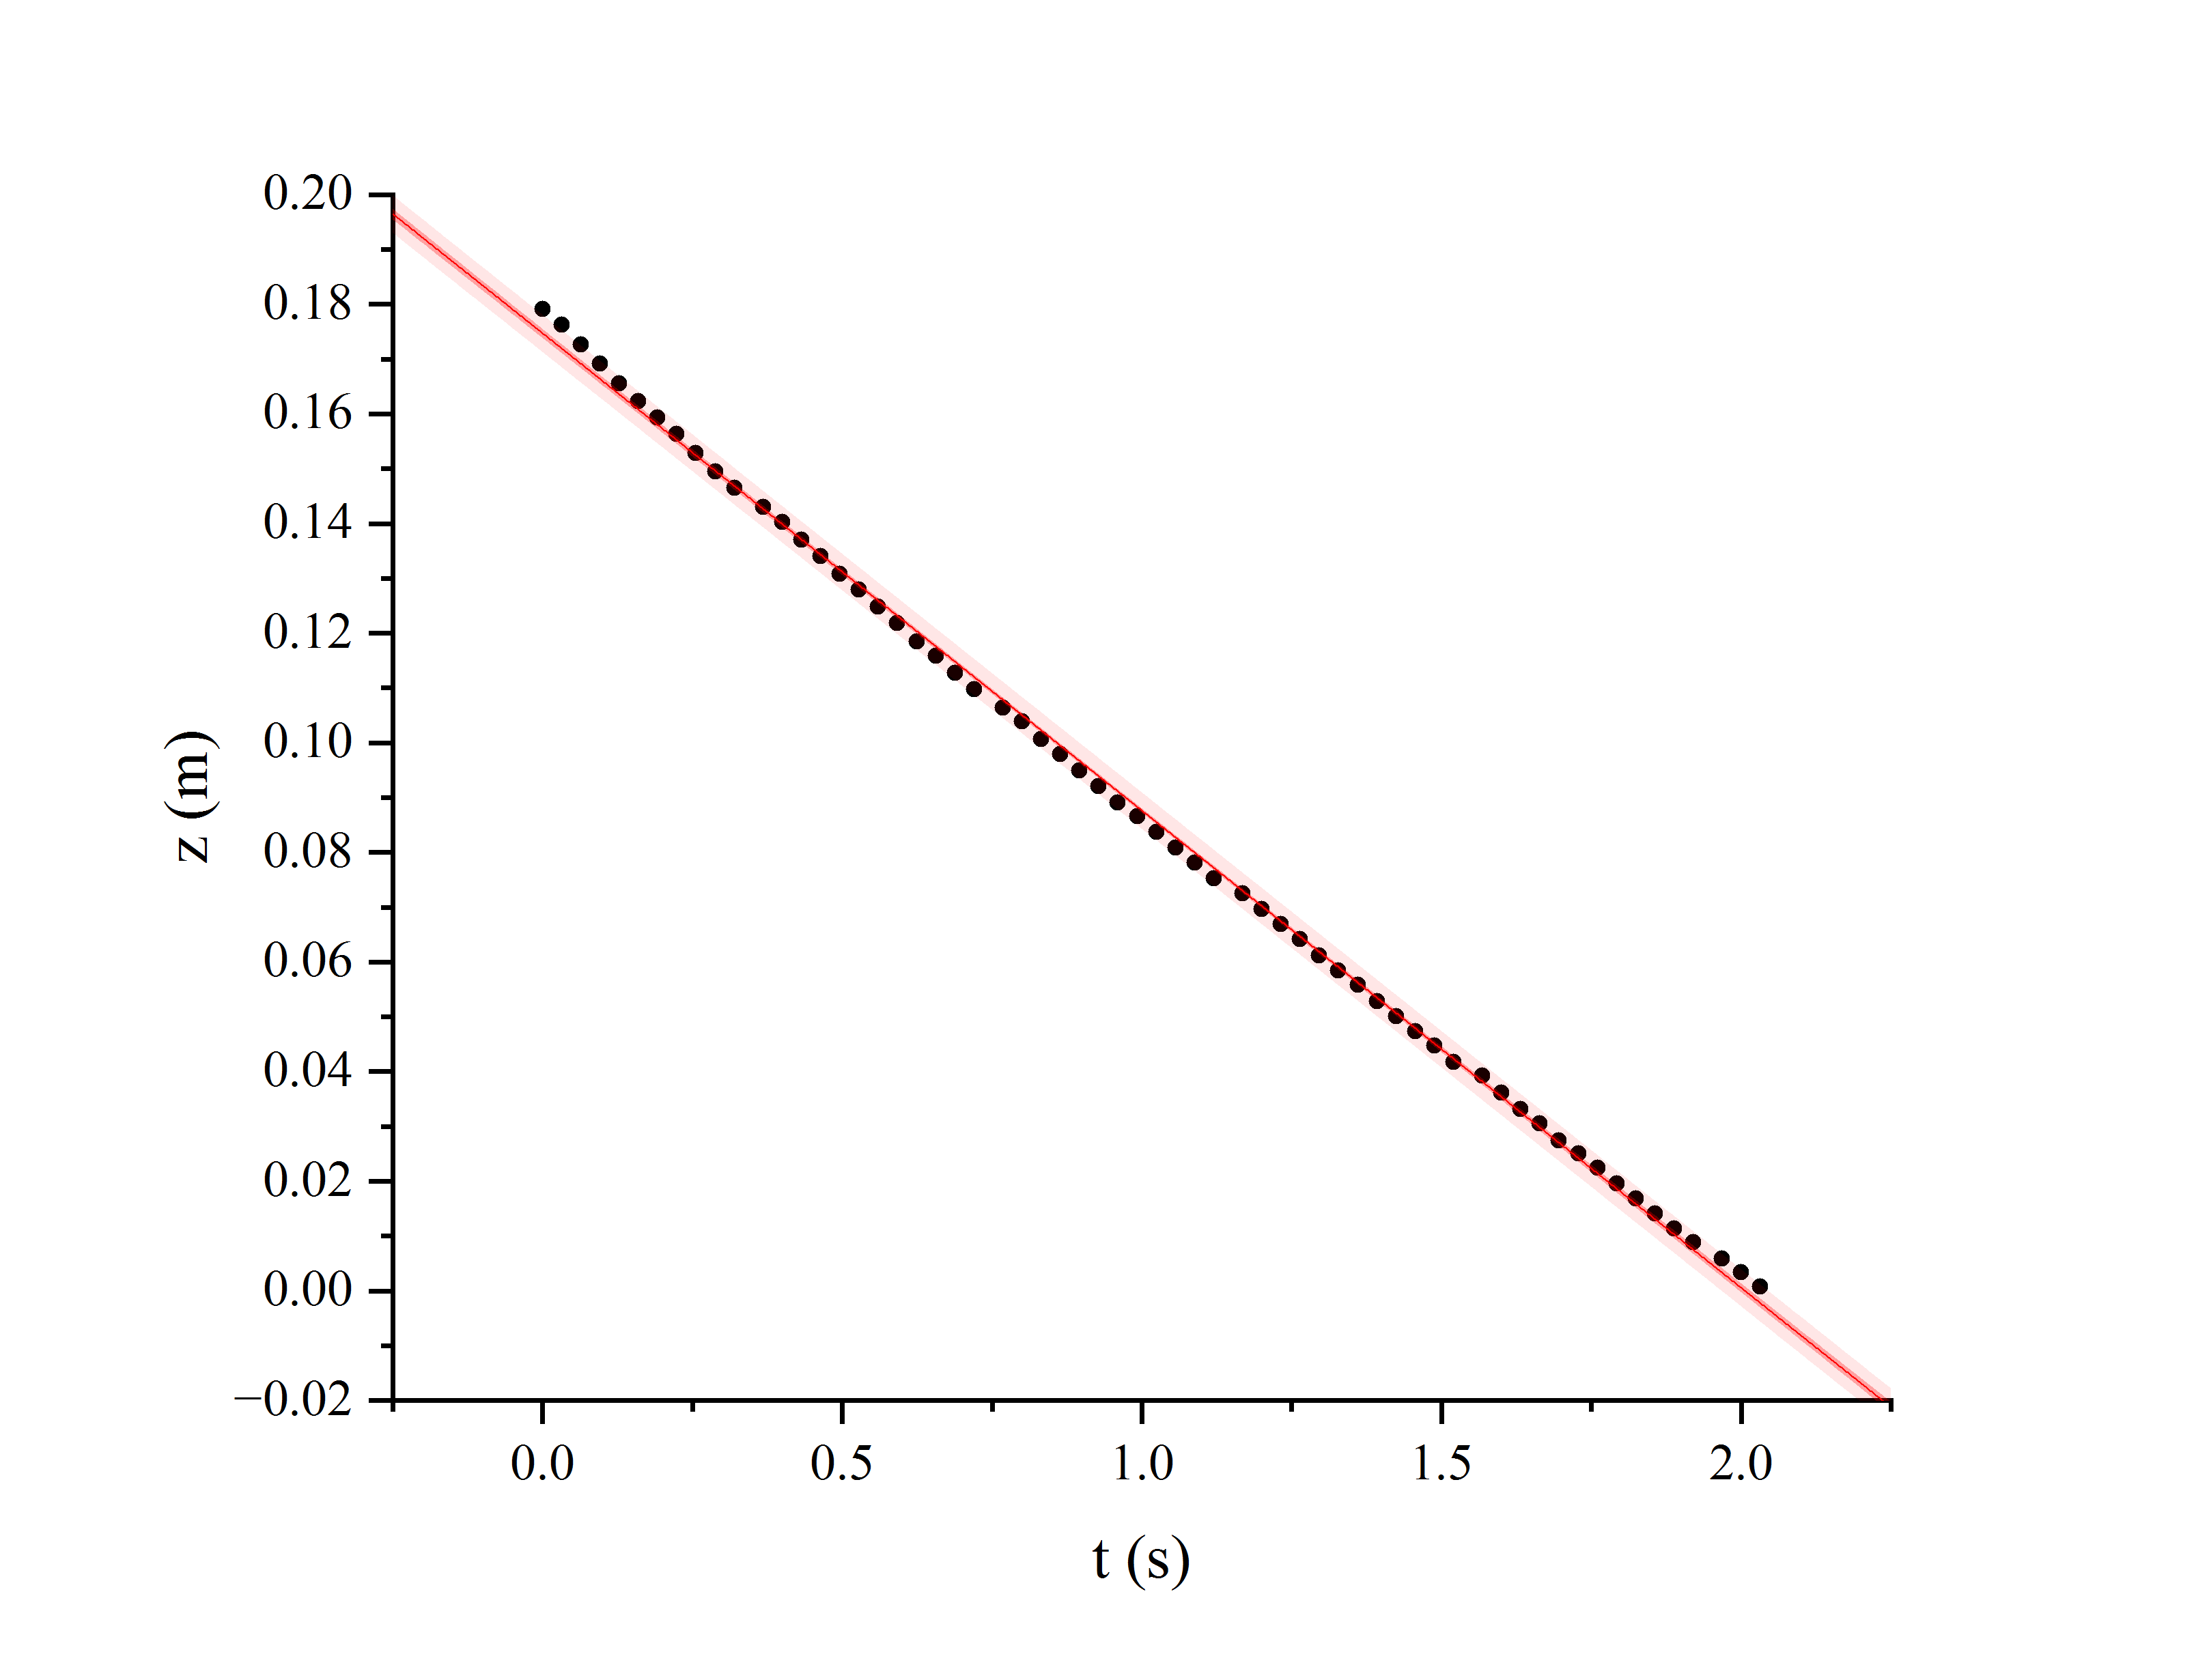
\includegraphics[trim={1.5cm 0.6cm 2cm 1cm},clip,width=\textwidth]{img/reg-p.png}
  \caption{\emph{
    In rosso la retta di regressione, in rosa la sua regione di incertezza.
  }}
\end{figure}

\emph{
  \textbf{Osservazione.} Come si può notare, l'andamento dei dati mostrati qui
  è ben descritto dalla retta: riteniamo che quindi, in questo caso, la sferetta
  abbia raggiunto la velocità limite prima di oltrepassare il primo traguardo.
}

\emph{
  Il gruppo di lavoro ha verificato in questo modo l'ipotesi (1.), osservando
  attentamente la distribuzione dei punti in ogni grafico: nessuno di questi
  ha mai mostrato una deviazione significativa dal modello lineare.
}

\pagebreak
Di seguito riportiamo le distribuzioni delle velocità per ogni classe
di sferette, di entrambi i giorni:
\vspace{-5mm}
\begin{center}
  \begin{figure}[H]
    % <v>^
    \centering
    \subfloat[][
      Primo giorno: piccole ($N=12$)

      $\overline{v}=(8.738\pm0.016)\cdot10^{-2}\,\unit{m\per s}$
    ]{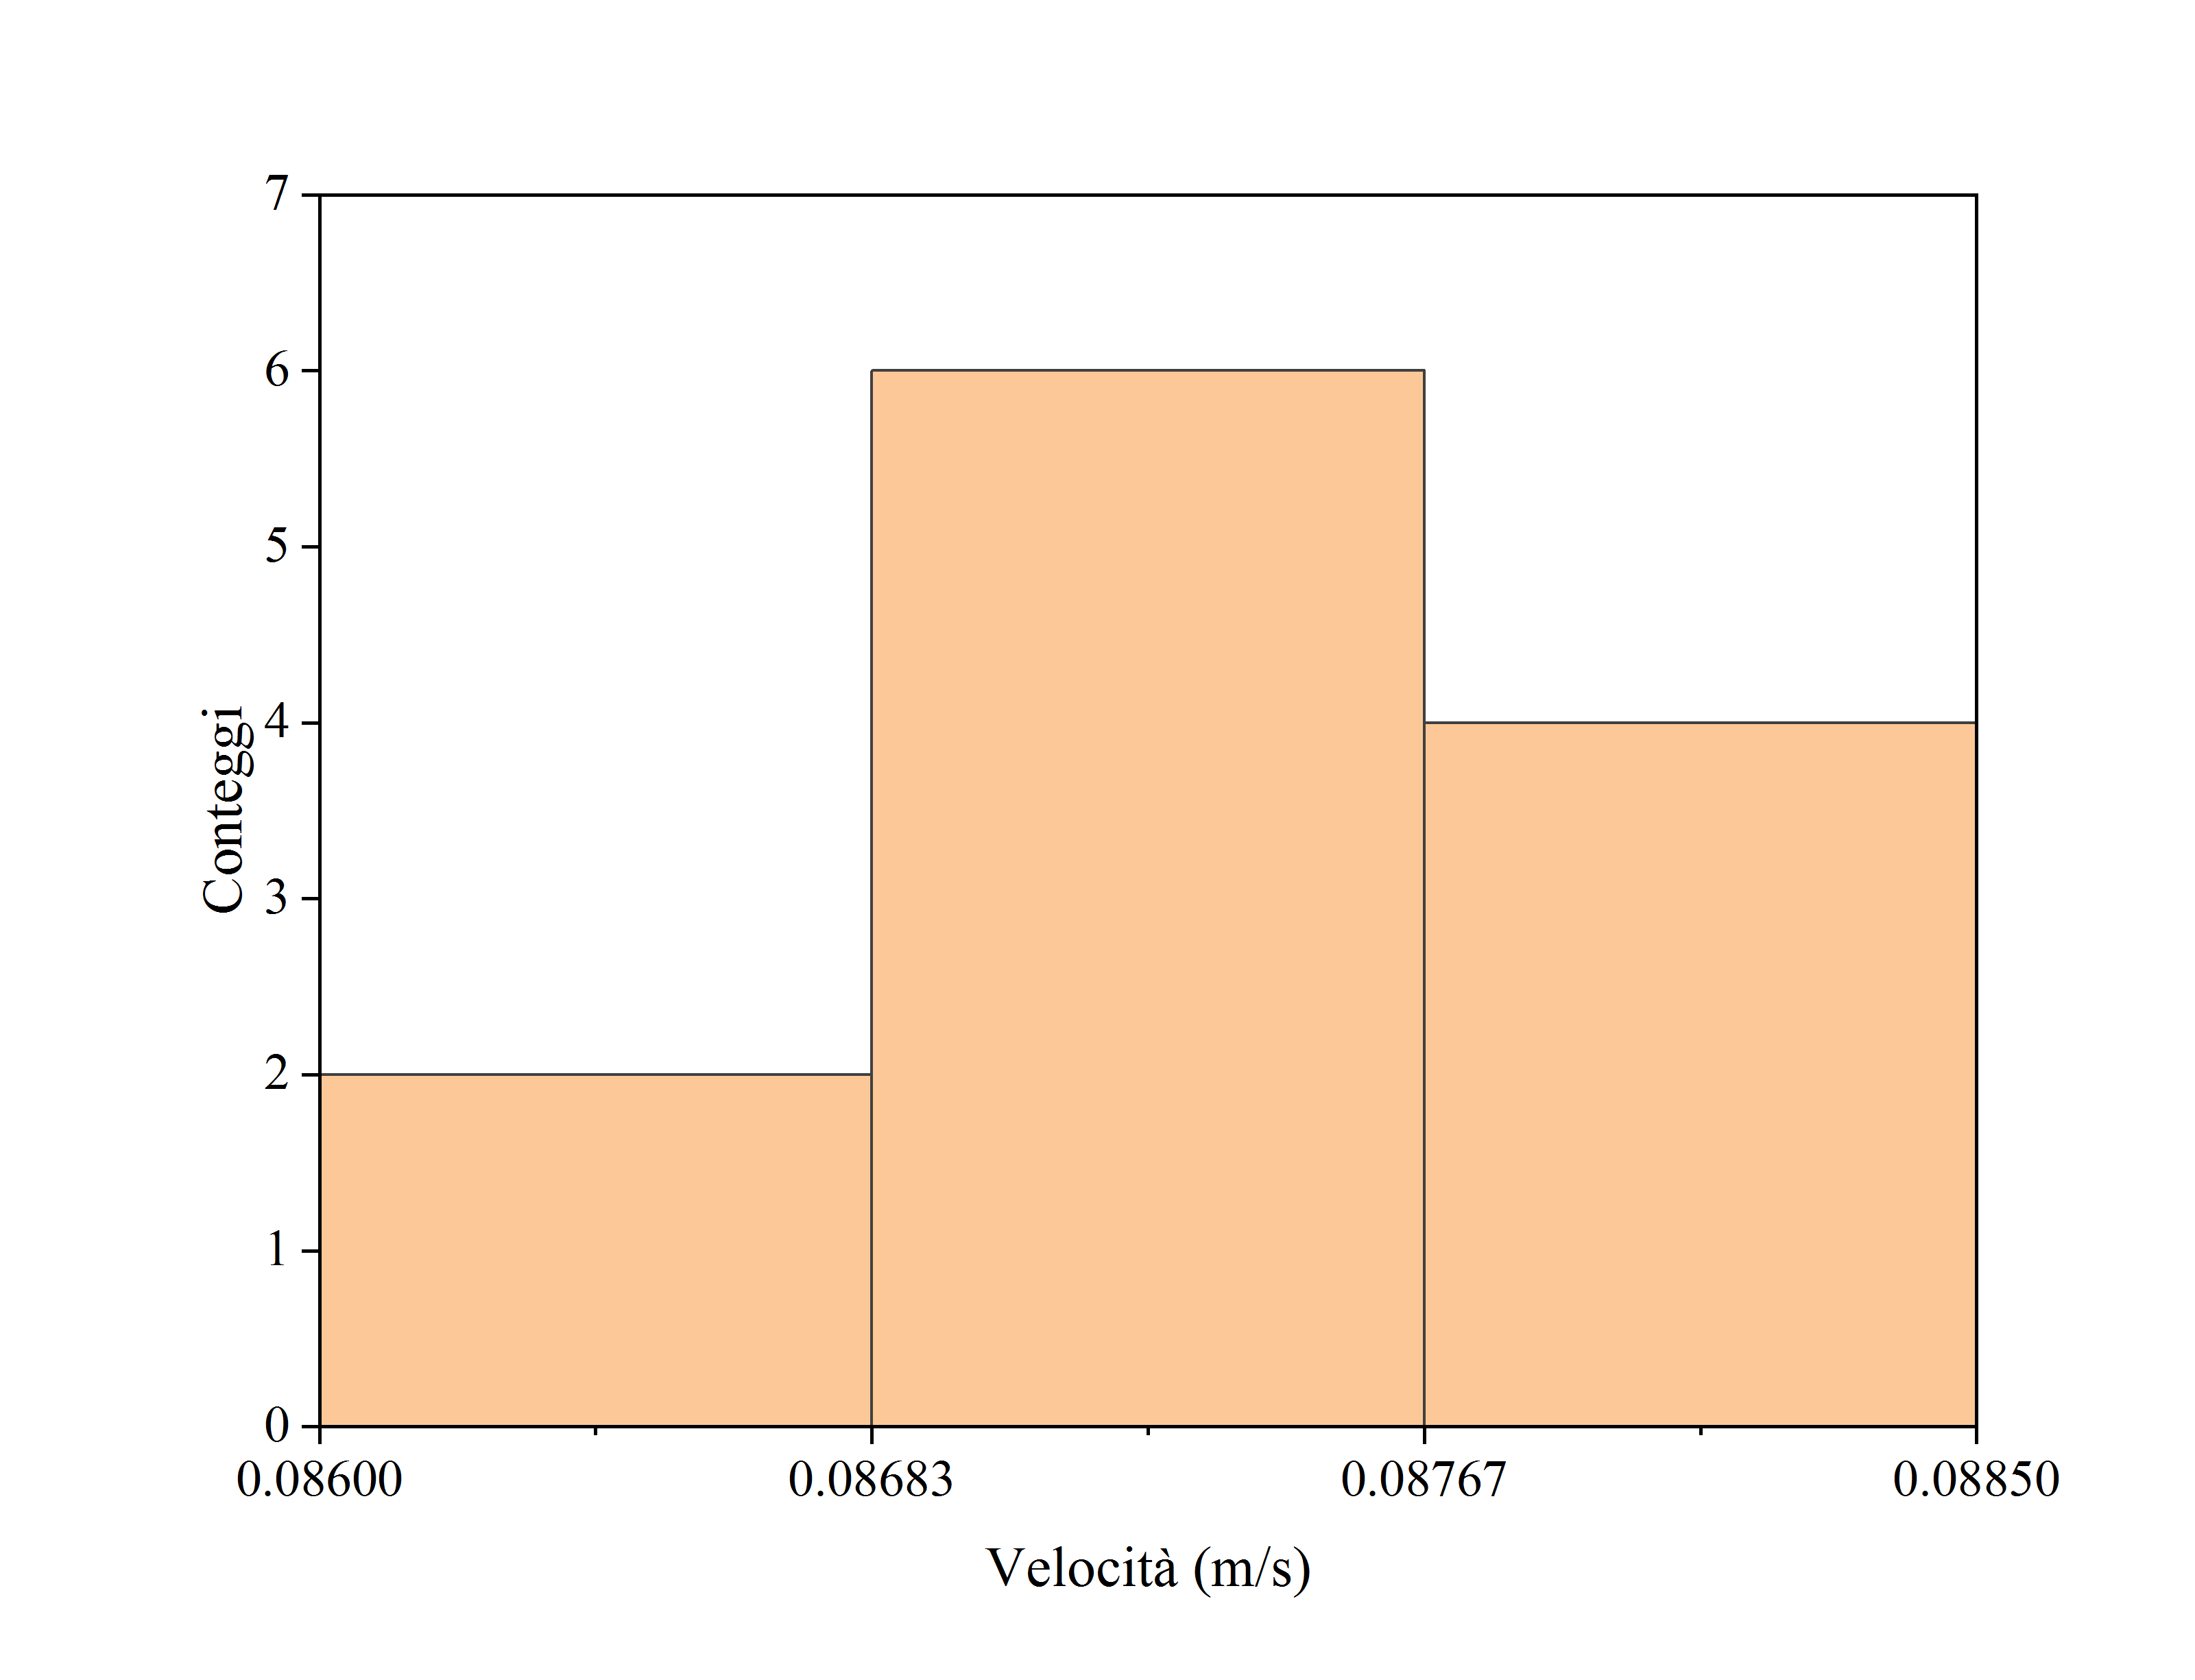
\includegraphics[trim={1cm 0.6cm 1cm 1cm},clip,width=.49\textwidth]{img/p1.png}}
    \hfil\subfloat[][
      Secondo giorno: piccole ($N=13$)

      $\overline{v}=(5.65\pm0.02)\cdot10^{-2}\,\unit{m\per s}$
    ]{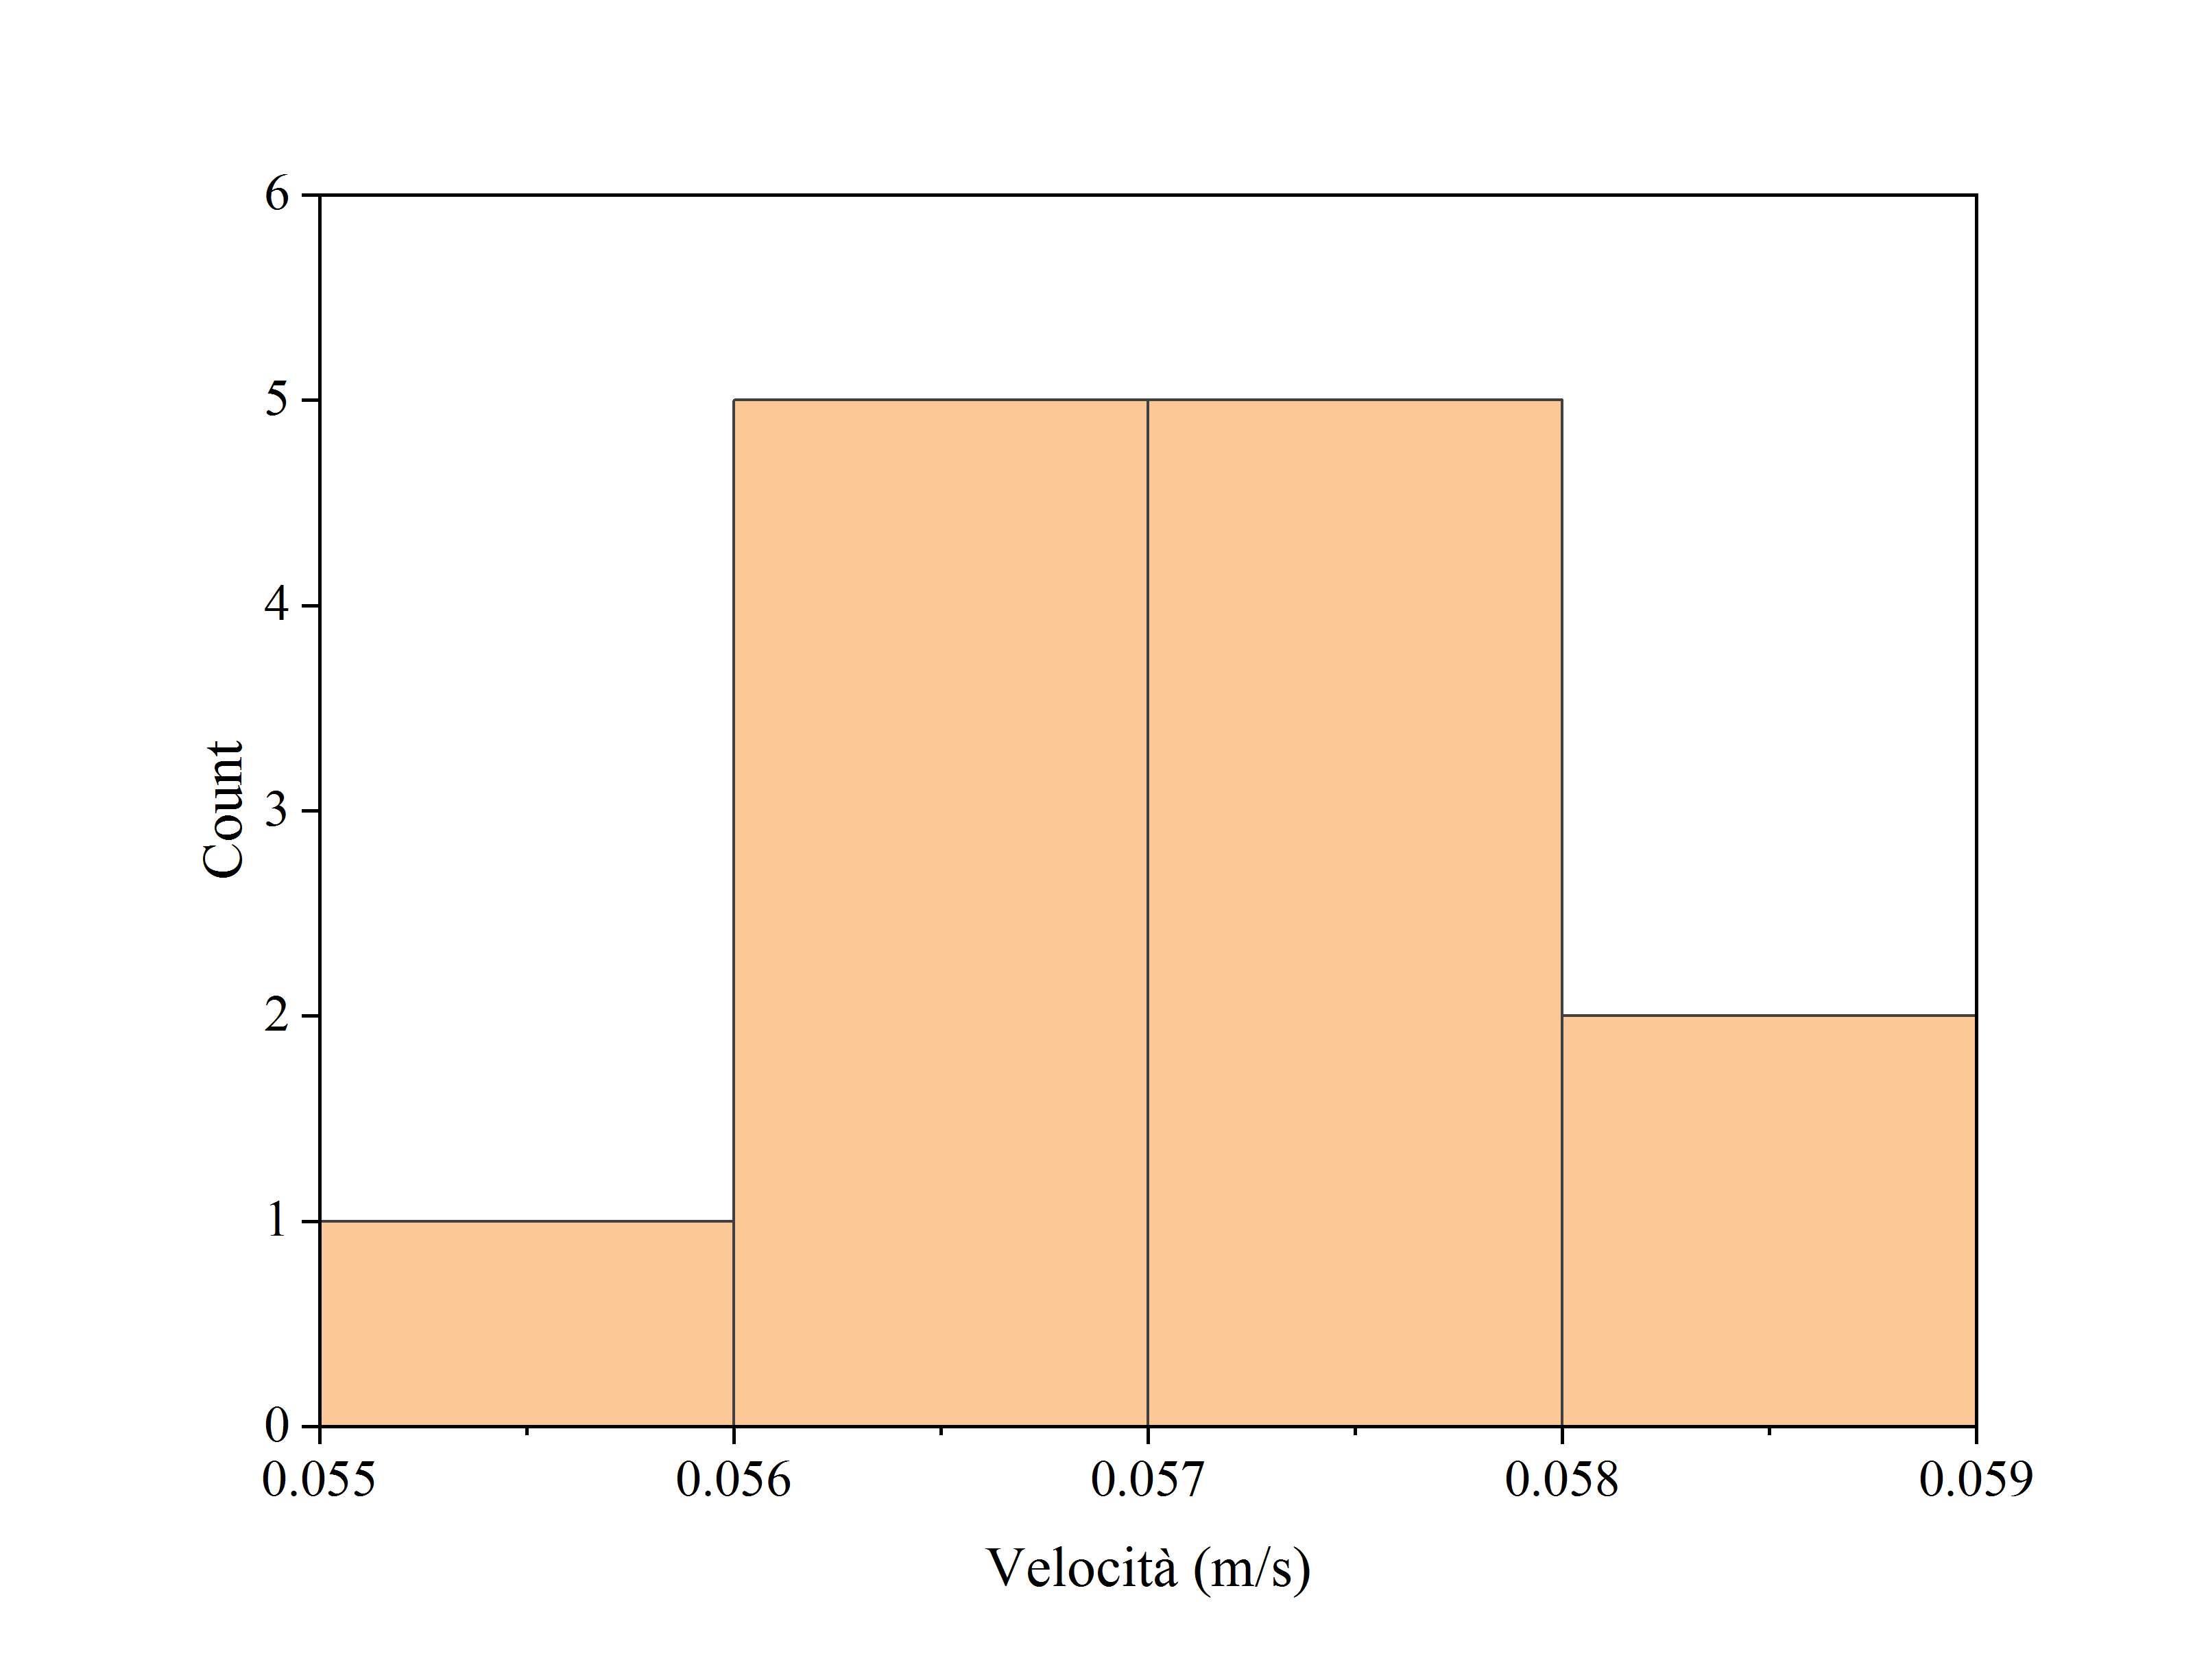
\includegraphics[trim={1cm 0.6cm 1cm 1cm},clip,width=.49\textwidth]{img/p2.png}}
    \hfil\subfloat[][
      Primo giorno: medie ($N=23$)

      $\overline{v}=(12.97\pm0.03)\cdot10^{-2}\,\unit{m\per s}$
    ]{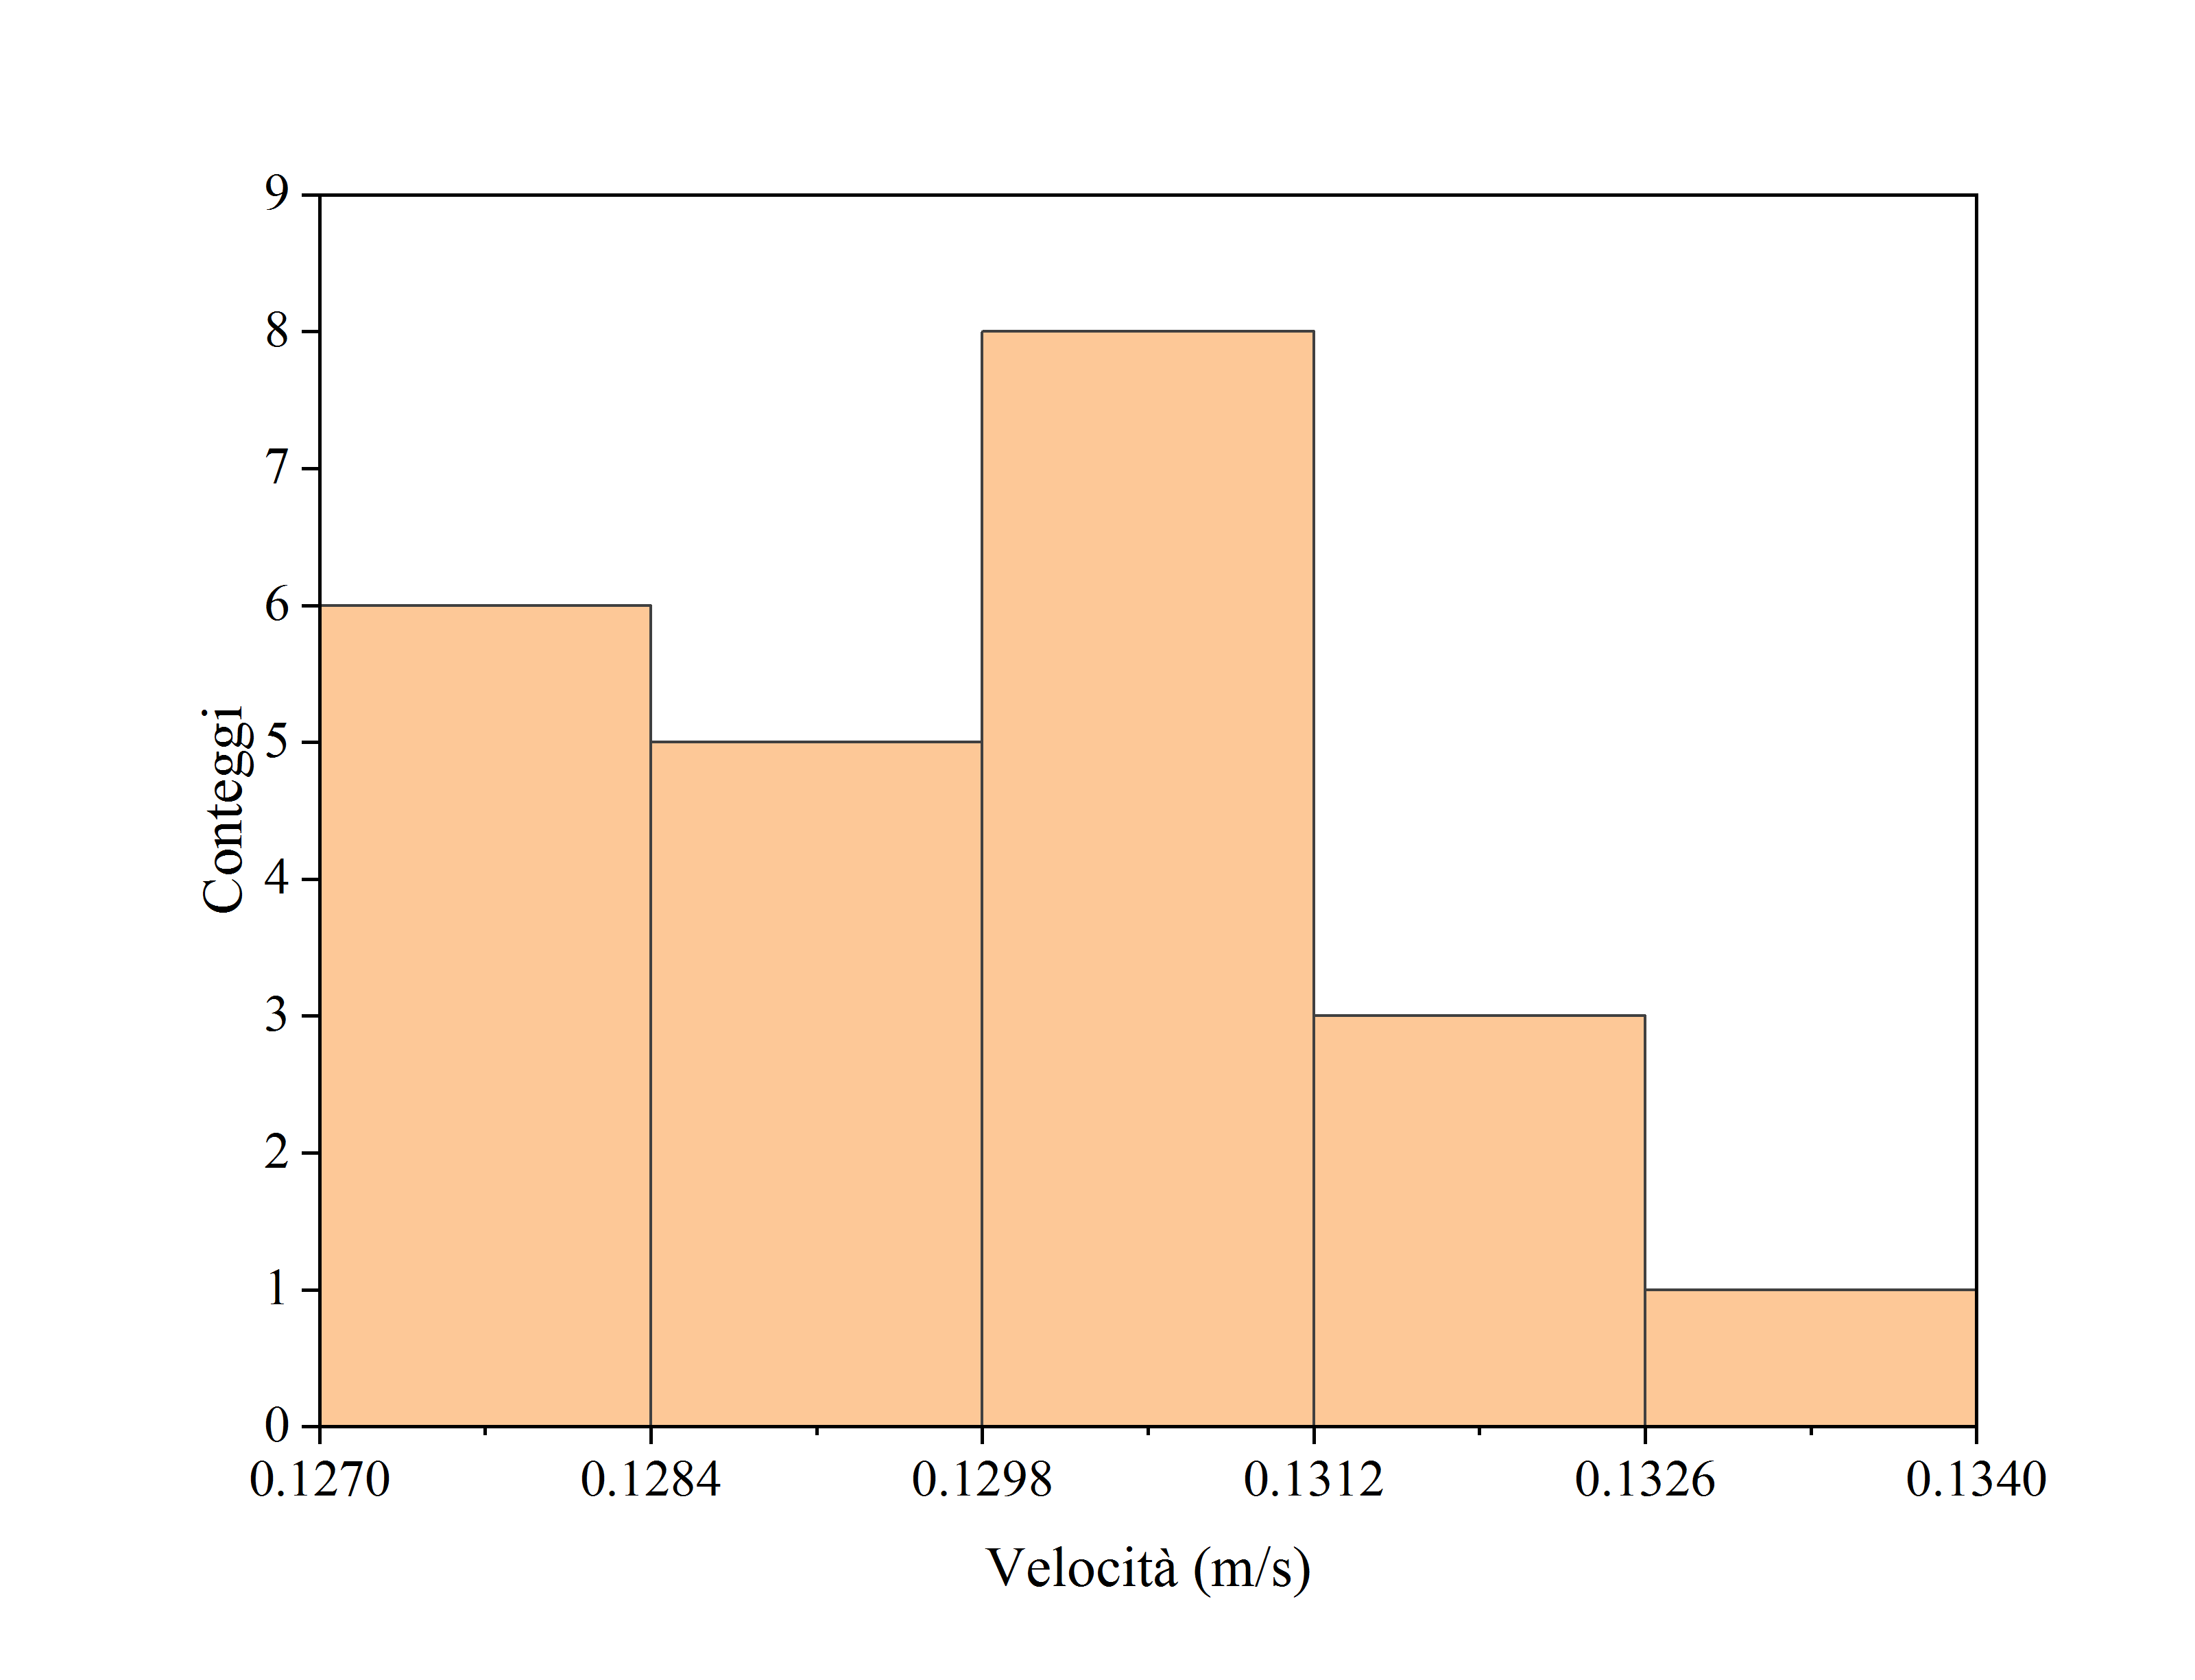
\includegraphics[trim={1cm 0.6cm 1cm 1cm},clip,width=.49\textwidth]{img/m1.png}}
    \hfil\subfloat[][
      Secondo giorno: medie ($N=23$)

      $\overline{v}=(8.61\pm0.04)\cdot10^{-2}\,\unit{m\per s}$
    ]{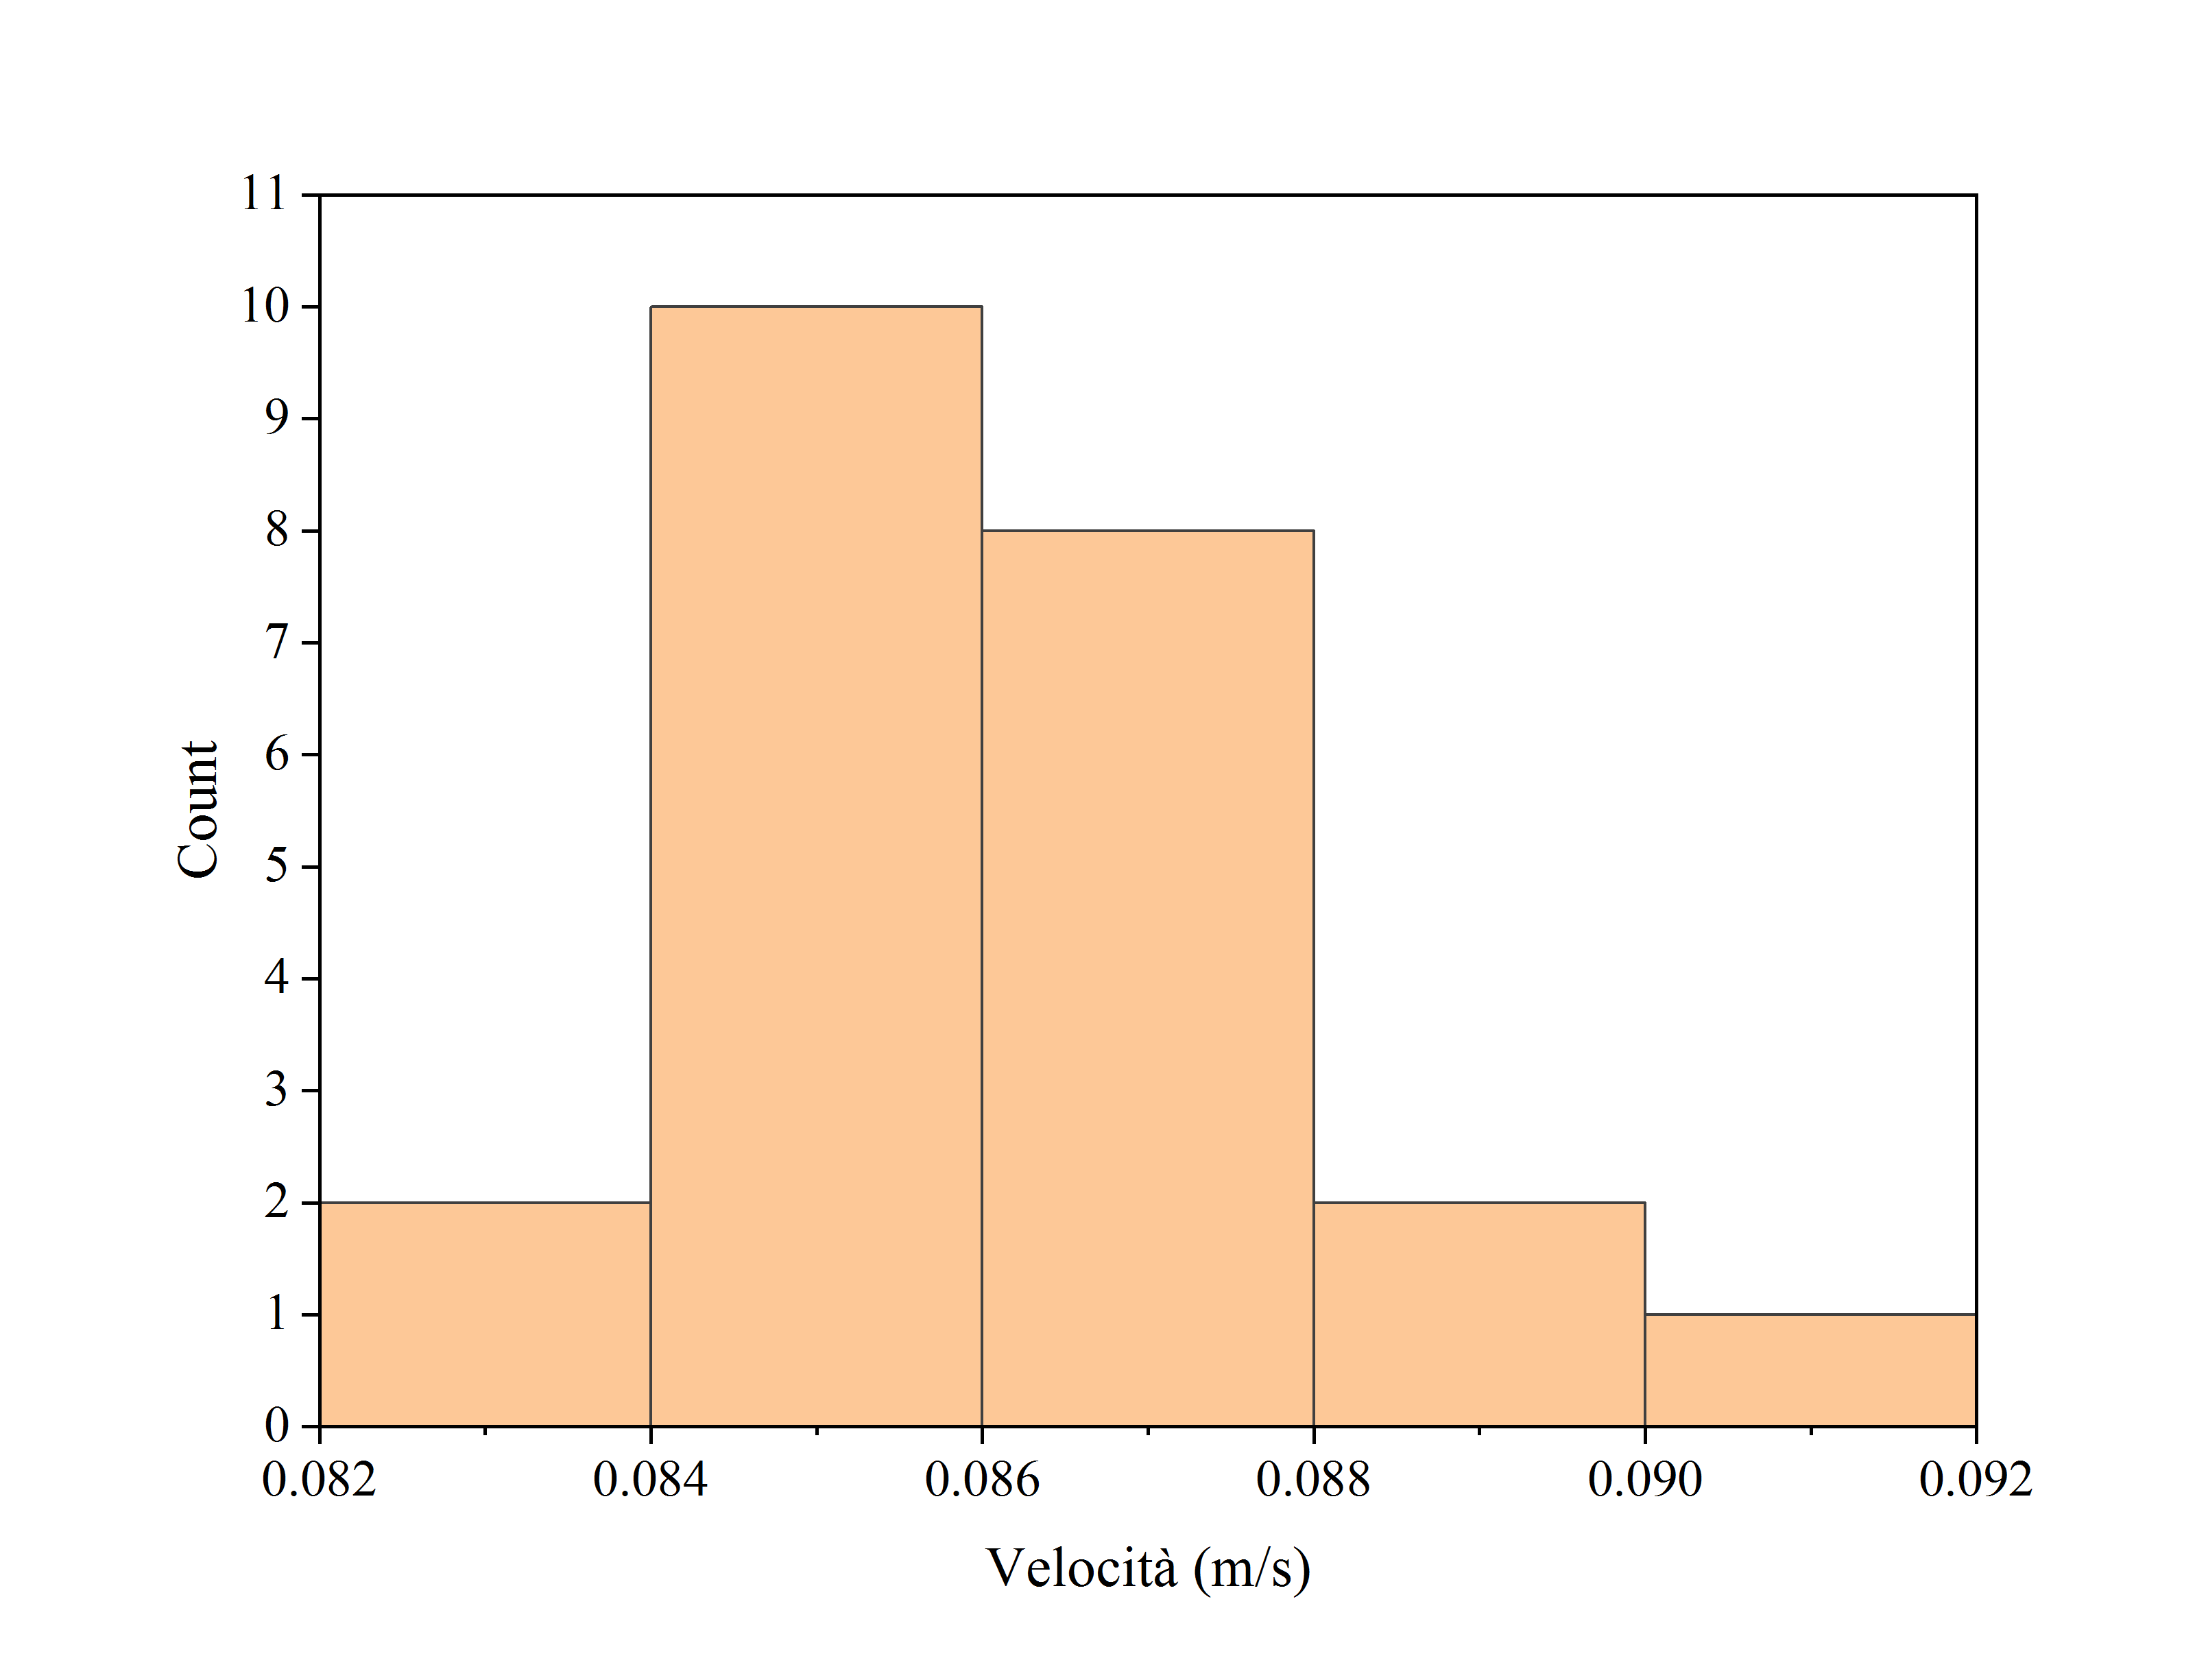
\includegraphics[trim={1cm 0.6cm 1cm 1cm},clip,width=.49\textwidth]{img/m2.png}}
    \hfil\subfloat[][
      Primo giorno: grandi ($N=32$)

      $\overline{v}=(19.58\pm0.05)\cdot10^{-2}\,\unit{m\per s}$
    ]{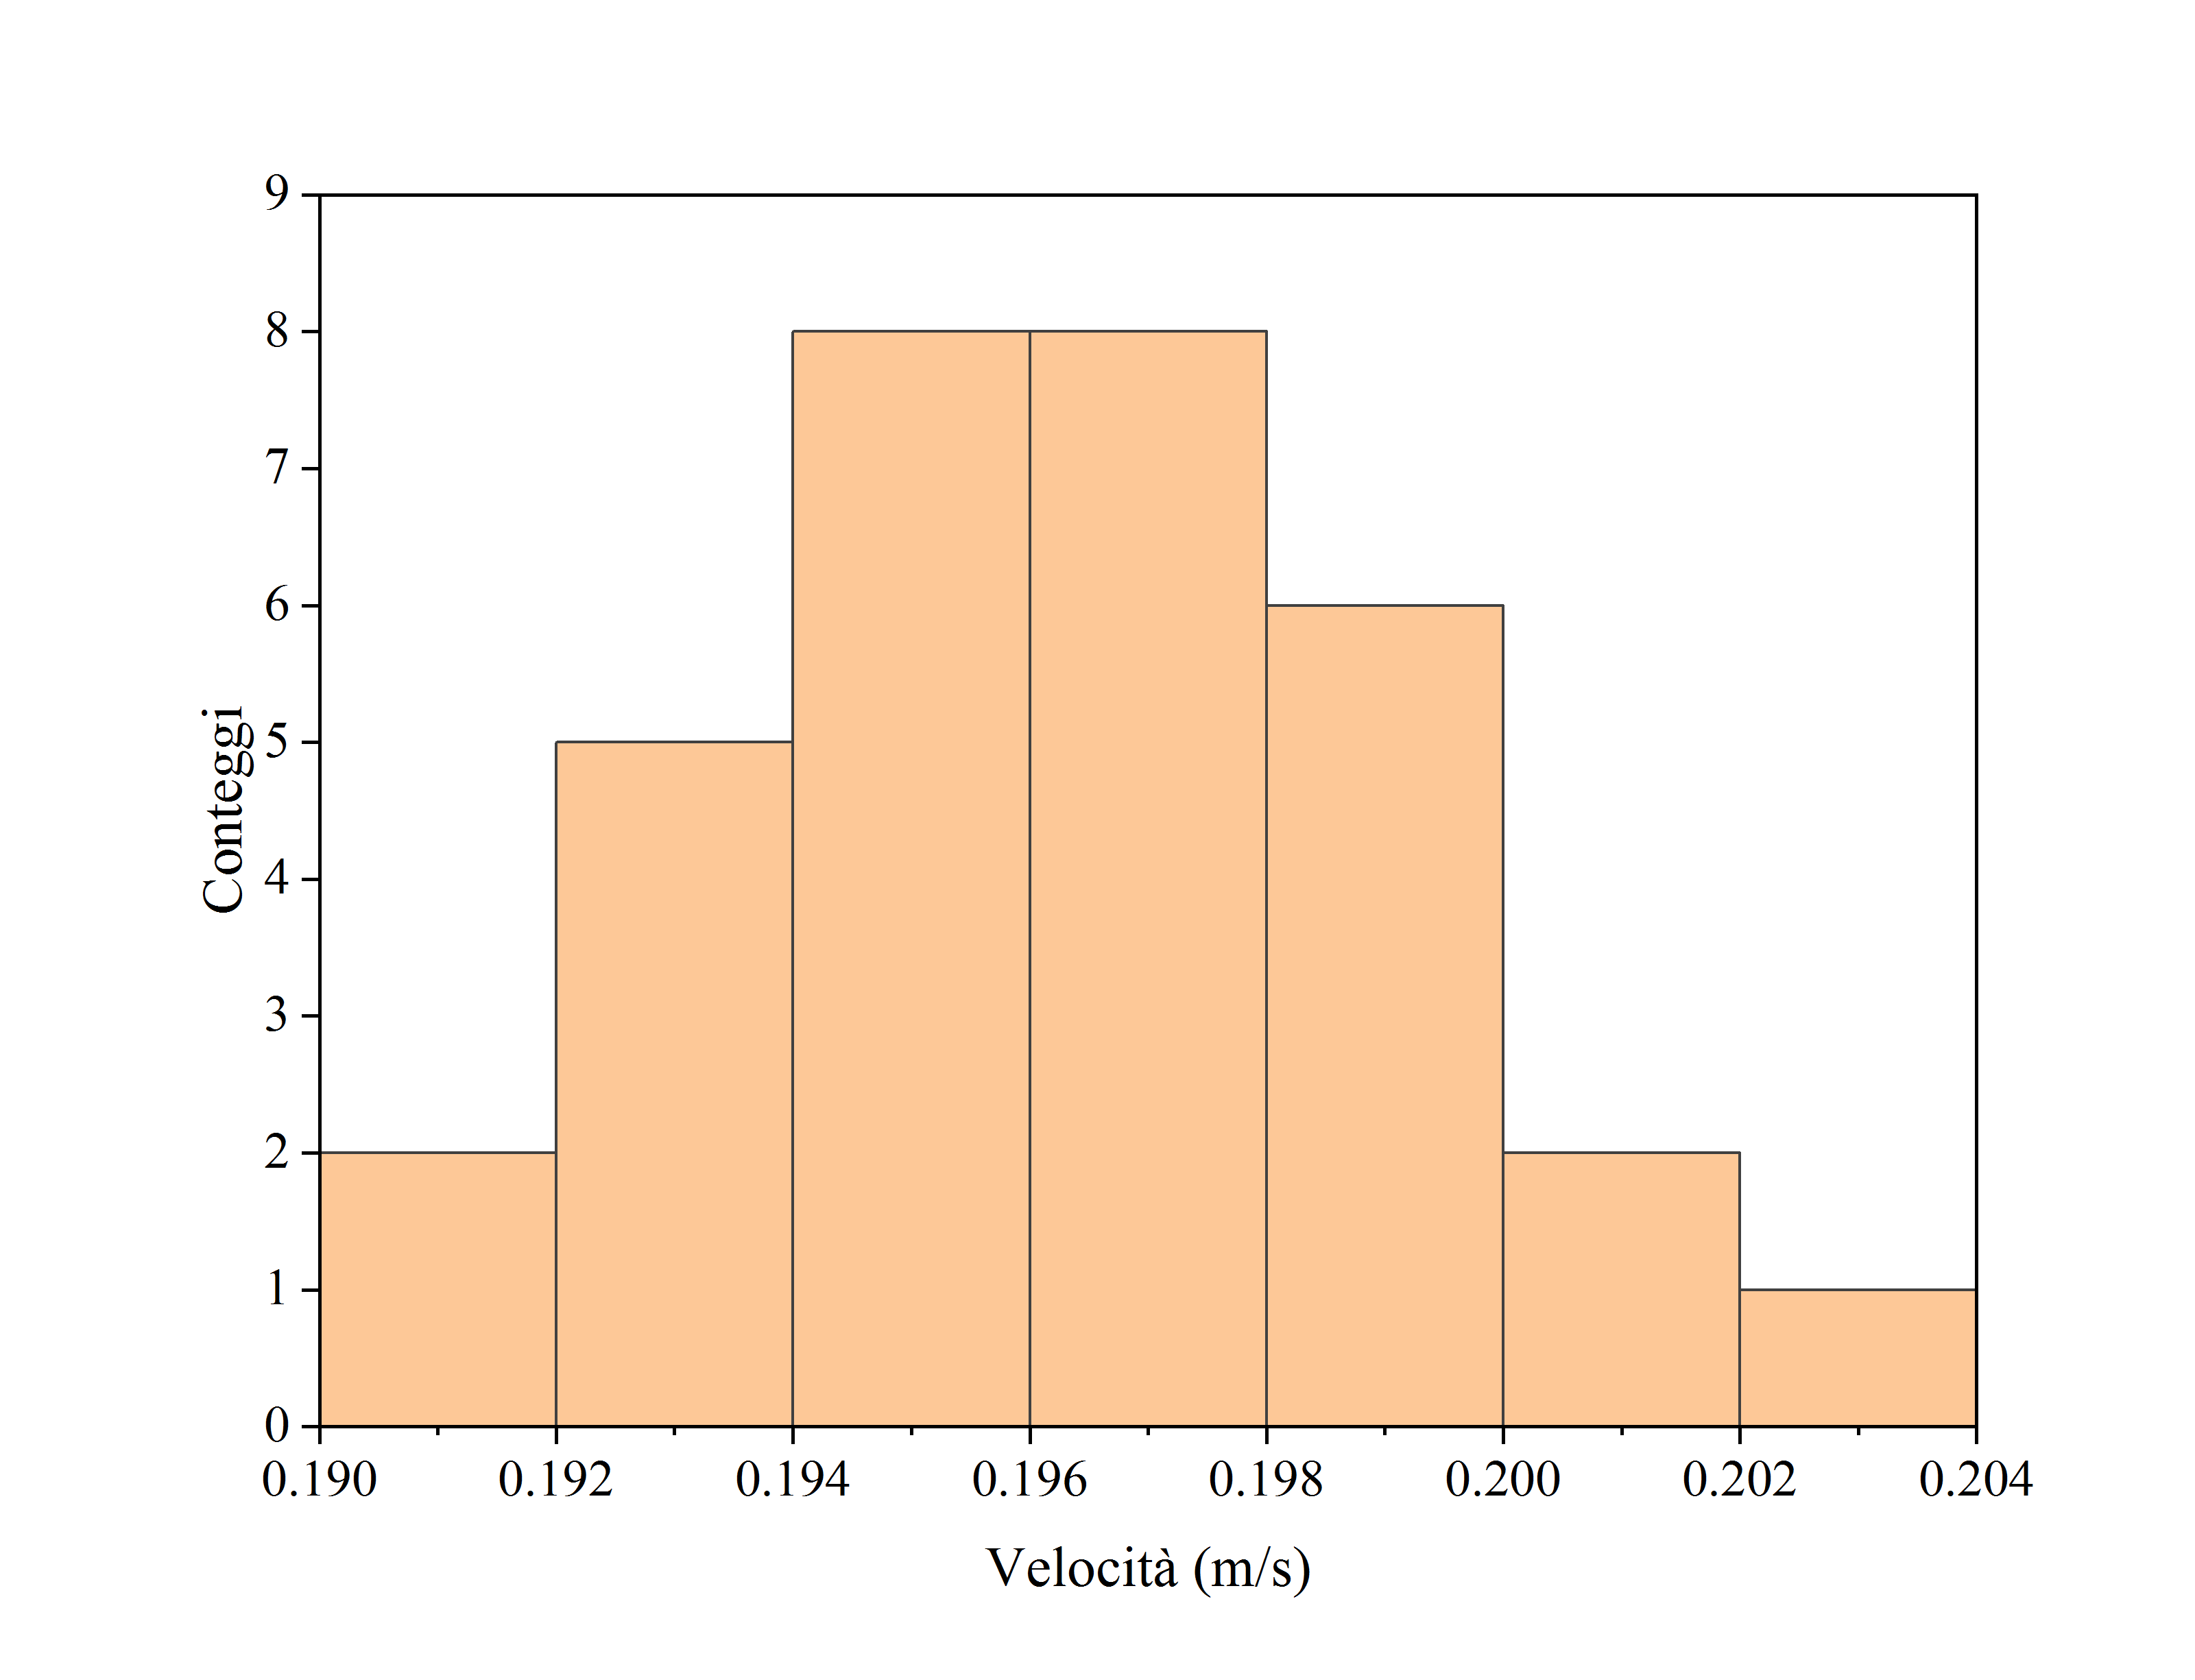
\includegraphics[trim={1cm 0.6cm 1cm 1cm},clip,width=.49\textwidth]{img/g1.png}}
    \hfil\subfloat[][
      Secondo giorno: grandi ($N=28$)

      $\overline{v}=(14.48\pm0.06)\cdot10^{-2}\,\unit{m\per s}$
    ]{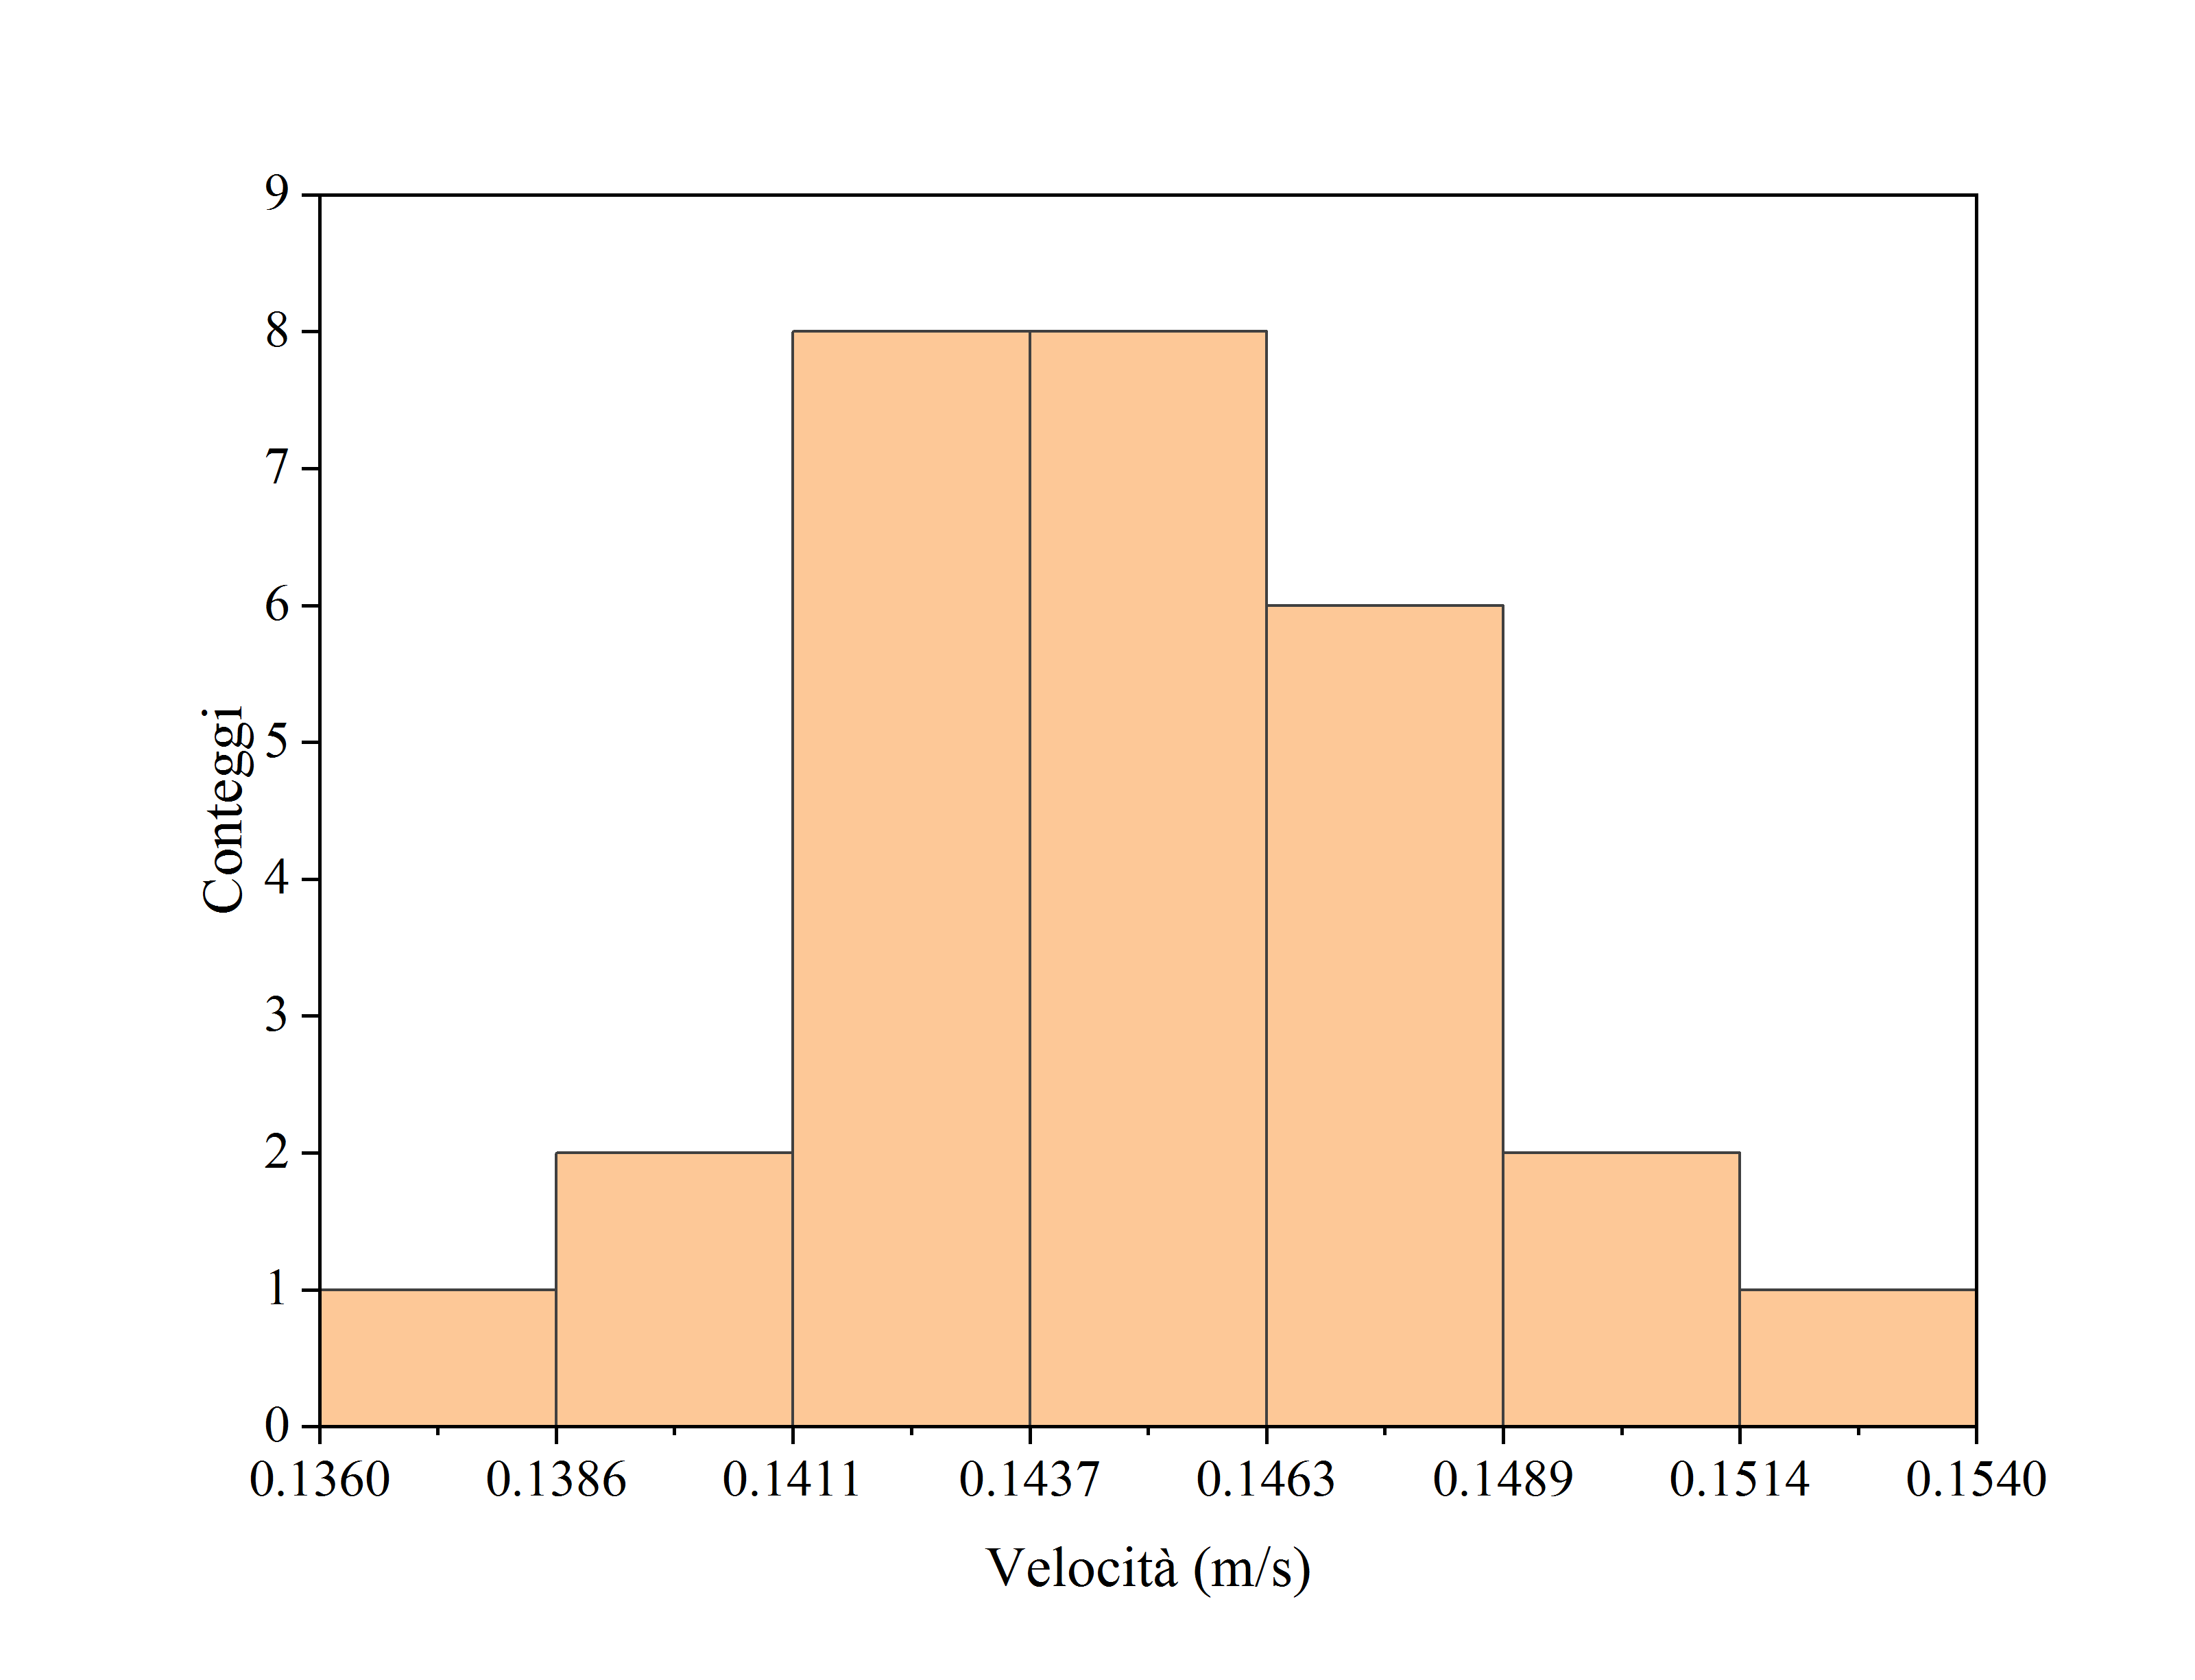
\includegraphics[trim={1cm 0.6cm 1cm 1cm},clip,width=.49\textwidth]{img/g2.png}}
  \end{figure}
\end{center}

\pagebreak
\textbf{Nota}.
Poiché la densità e la viscosità della soluzione,
ma in generale di un fluido reale, dipendono dalla temperatura,
il gruppo di lavoro ha ritenuto opportuno
applicare un modello empirico, in particolare quello sviluppato
da N.S.Cheng\cite{Cheng2008} nel 2008 e da A. Volk e C. J.
K\"ahler\cite{Volk2018} nel 2018.

Si noti che questo modello è applicabile, come specificato dagli
autori, a temperature nell'intervallo
$\left(\qty{0}{\degree C},\qty{100}{\degree C}\right)$,
nel quale le temperature ambientali misurate ($T_\text{amb}$)
rientrano abbondantemente.

\subsection{Modello di $\rho(T)$ ed $\eta(T)$ per i liquidi puri}
Il modello di cui sopra descrive molto bene densità e viscosità
di acqua e glicerina (pure), in funzione della temperatura,
mediante queste relazioni:
\[\begin{aligned}
  \eta_\text{acqua}(T\,\,\unit{\degree C}) &= 1.79\cdot\exp{\!\left(
    \frac{-(1230 + T)\cdot T}{36100 + 360\,T}
  \right)}\,\unit{mPa\,s} \\
  \eta_\text{glicerina}(T\,\,\unit{\degree C}) &= 12100\cdot\exp{\!\left(
    \frac{-(1233 + T)\cdot T}{9900 + 70\,T}\right)}\,\unit{mPa\,s} \\
  \rho_\text{acqua}(T\,\,\unit{\degree C}) &= 1000 \left(
    1 - \left|\frac{T - 3.98}{615}\right|^{1.71} \right)\,\unit{kg \per m^3} \\
  \rho_\text{glicerina}(T\,\,\unit{\degree C}) &= \left(
    1273 - 0.612\,T \right)\,\unit{kg \per m^3}
\end{aligned}\]

Di seguito riportiamo i valori di queste grandezze, calcolati alle
due temperature $T_{\text{amb},1}$ e $T_{\text{amb},2}$:
\begin{center}
\begin{tblr}{
  colspec={ |cc|c|c| },
}
  \hline
  $T_{\text{amb}}$ & $(\unit{\degree C})$
    & $24.6\pm0.2$ & $19.4\pm0.2$ \\
  \hline
  $\eta_\text{acqua}$ & $(\unit{mPa\,s})$
    & $0.901\pm0.004$ & $1.020\pm0.005$ \\
  \hline[dashed]
  $\eta_\text{glicerina}$ & $(\unit{mPa\,s})$
    & $845\pm16$ & $1398\pm28$ \\
  \hline[dashed]
  $\rho_\text{acqua}$ & $(\unit{kg \per m^3})$
    & $996.99\pm0.05$ & $998.17\pm0.04$ \\
  \hline[dashed]
  $\rho_\text{glicerina}$ & $(\unit{kg \per m^3})$
    & $1257.94\pm0.12$ & $1261.13\pm0.12$ \\
  \hline
\end{tblr}
\end{center}

\subsection{Misura di $\eta_\text{sol}$}
Ricordiamo la relazione tra $\overline{v}_k$ e $\overline{r}_k^2$:
\[
  \overline{v}_k = \xi\cdot\overline{r}_k^2
  \qquad\qquad\text{avendo posto}\qquad
  \xi = \frac{2g(\rho_\text{sf} - \rho_\text{sol})}{9\eta_\text{sol}}
\]
Trattandosi di una relazione lineare, è possibile determinare una
retta di regressione, nella quale, poiché il modello lo richiedeva,
abbiamo fissato l'intercetta a 0.
Chiaramente, i dati dei due giorni devono essere trattati separatamente,
poiché $\rho_\text{sol}$ ed $\eta_\text{sol}$ dipendono dalla temperatura
ambiente.

Di seguito riportiamo i due grafici così ottenuti:

\vspace{-2mm}
\begin{figure}[H]
  \centering
  \subfloat[][
    Primo giorno

    $\xi=(8.738\pm0.016)\cdot10^{-2}\,\unit{m\cdot s}$
  ]{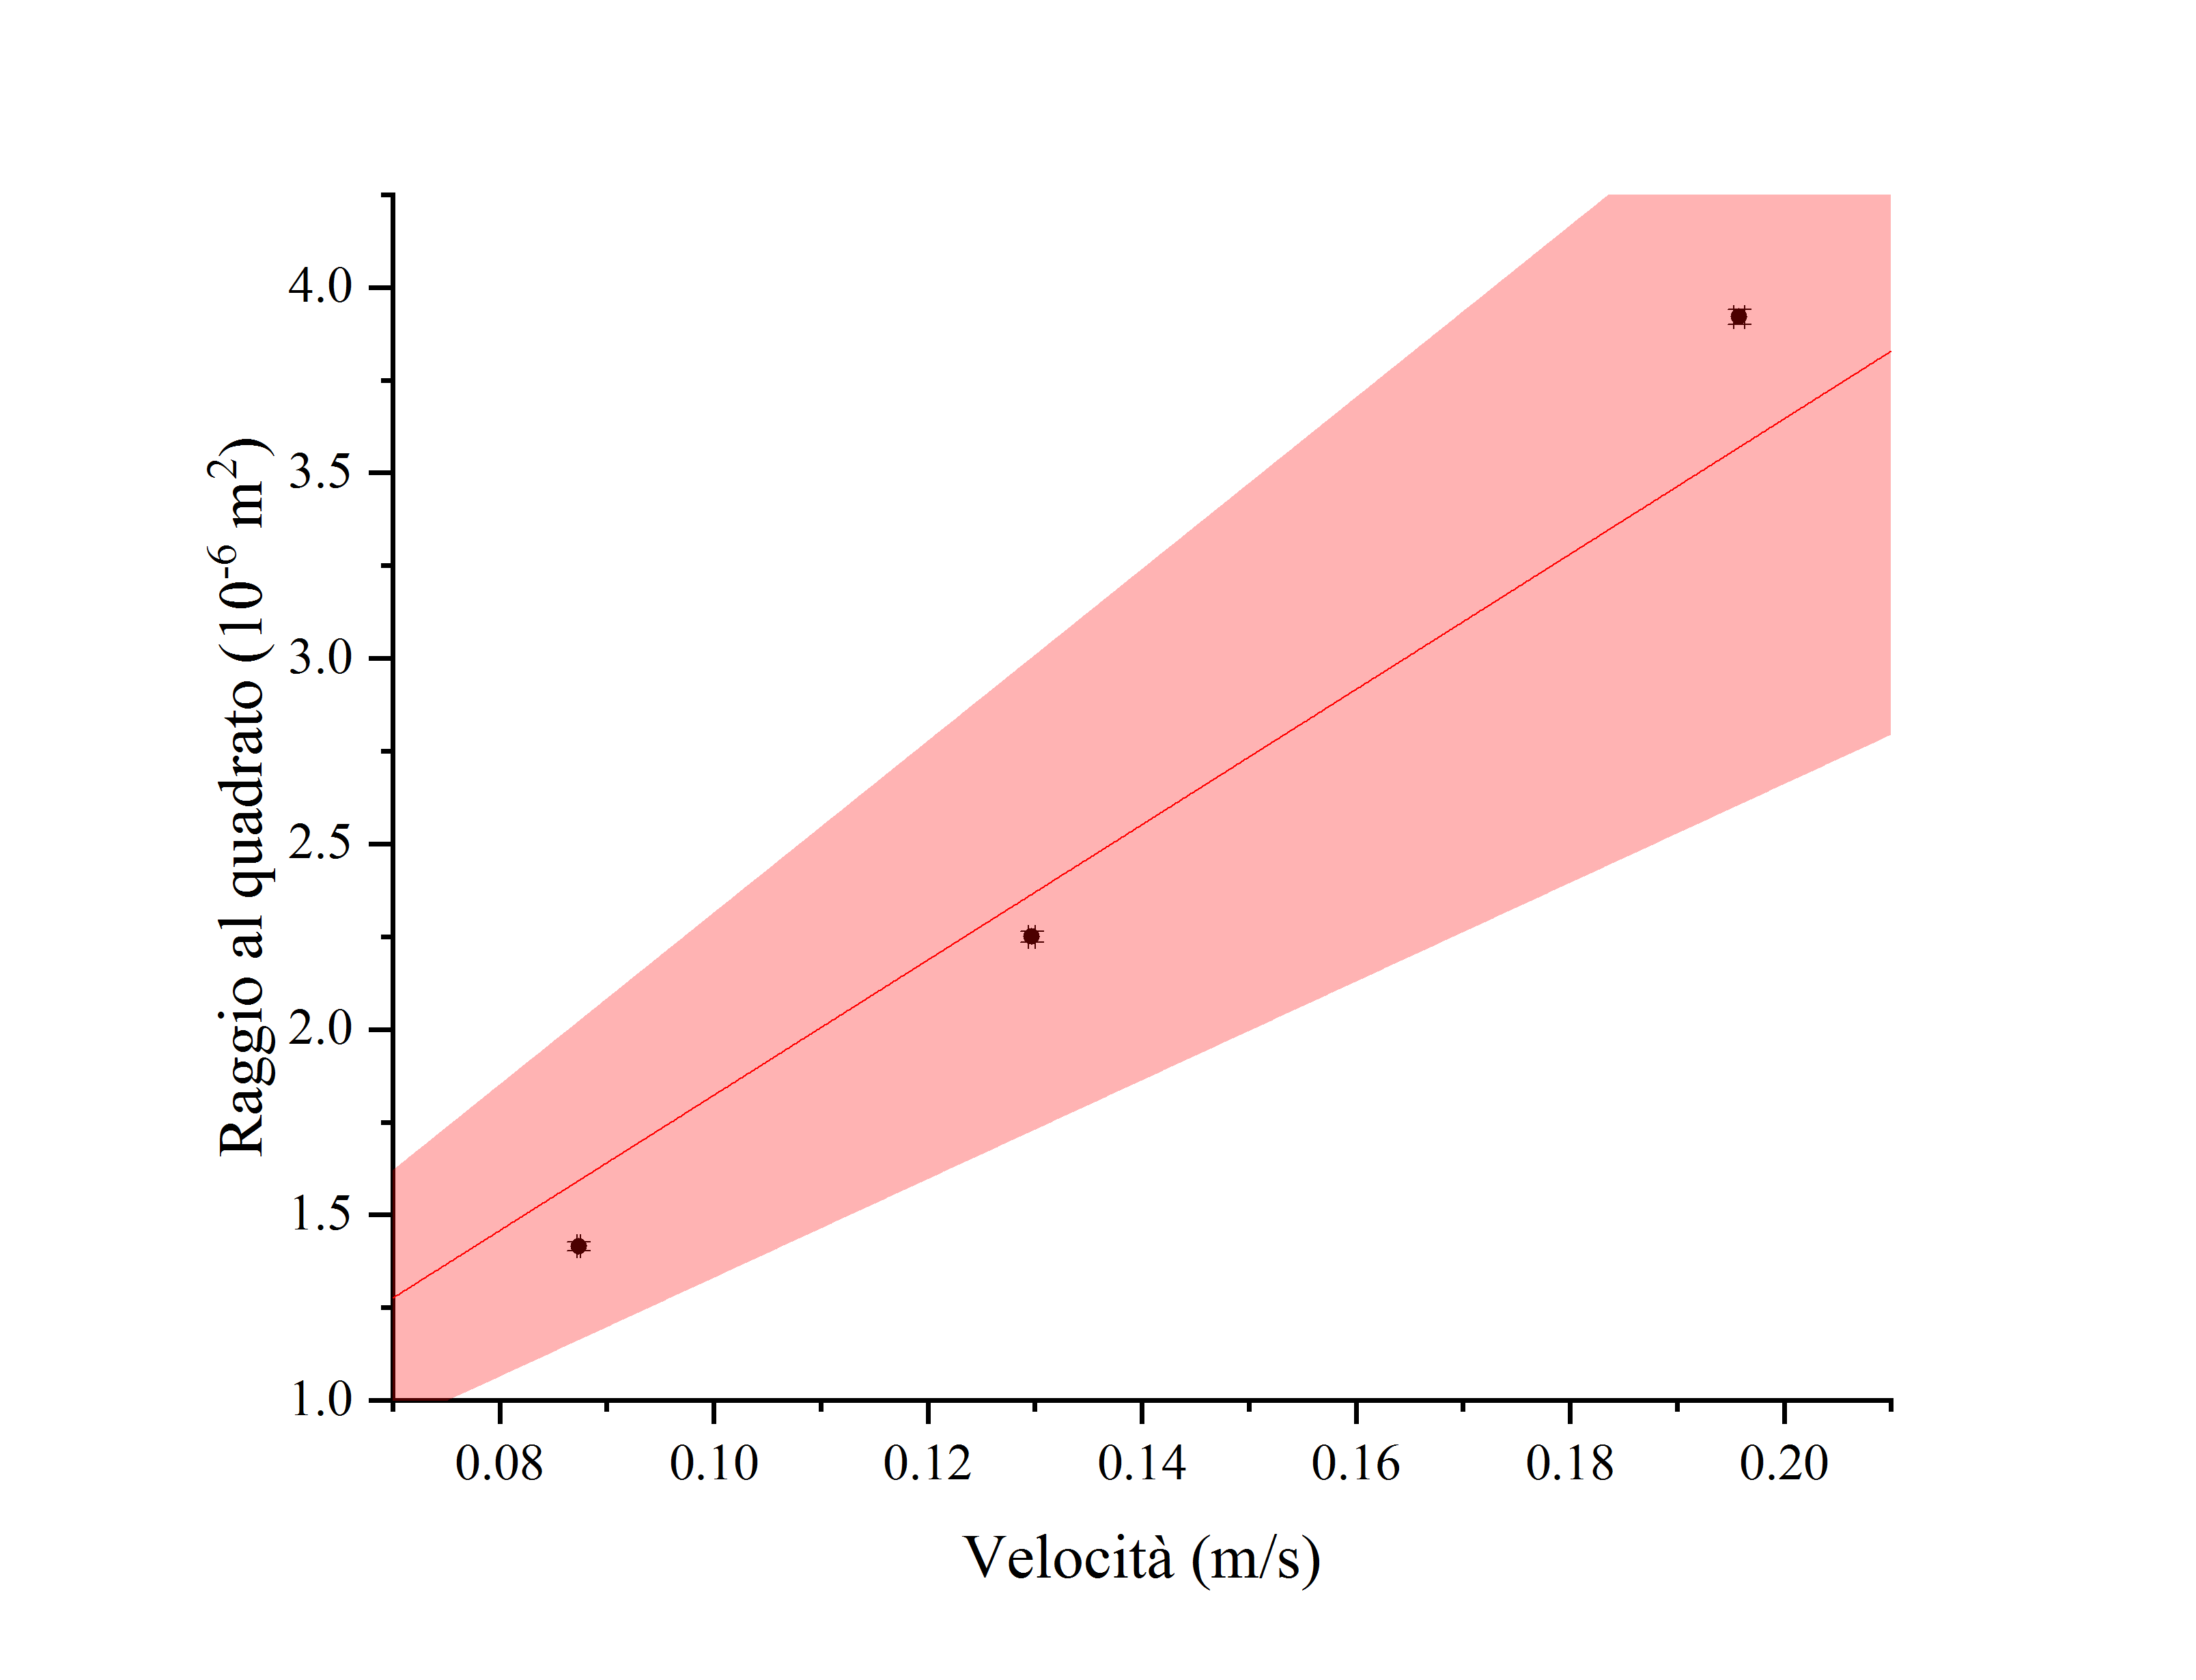
\includegraphics[trim={2.5cm 0.6cm 2.5cm 2.5cm},clip,width=.49\textwidth]{img/reg1.png}}
  \hfil\subfloat[][
    Secondo giorno

    $\xi=(5.65\pm0.02)\cdot10^{-2}\,\unit{m\cdot s}$
  ]{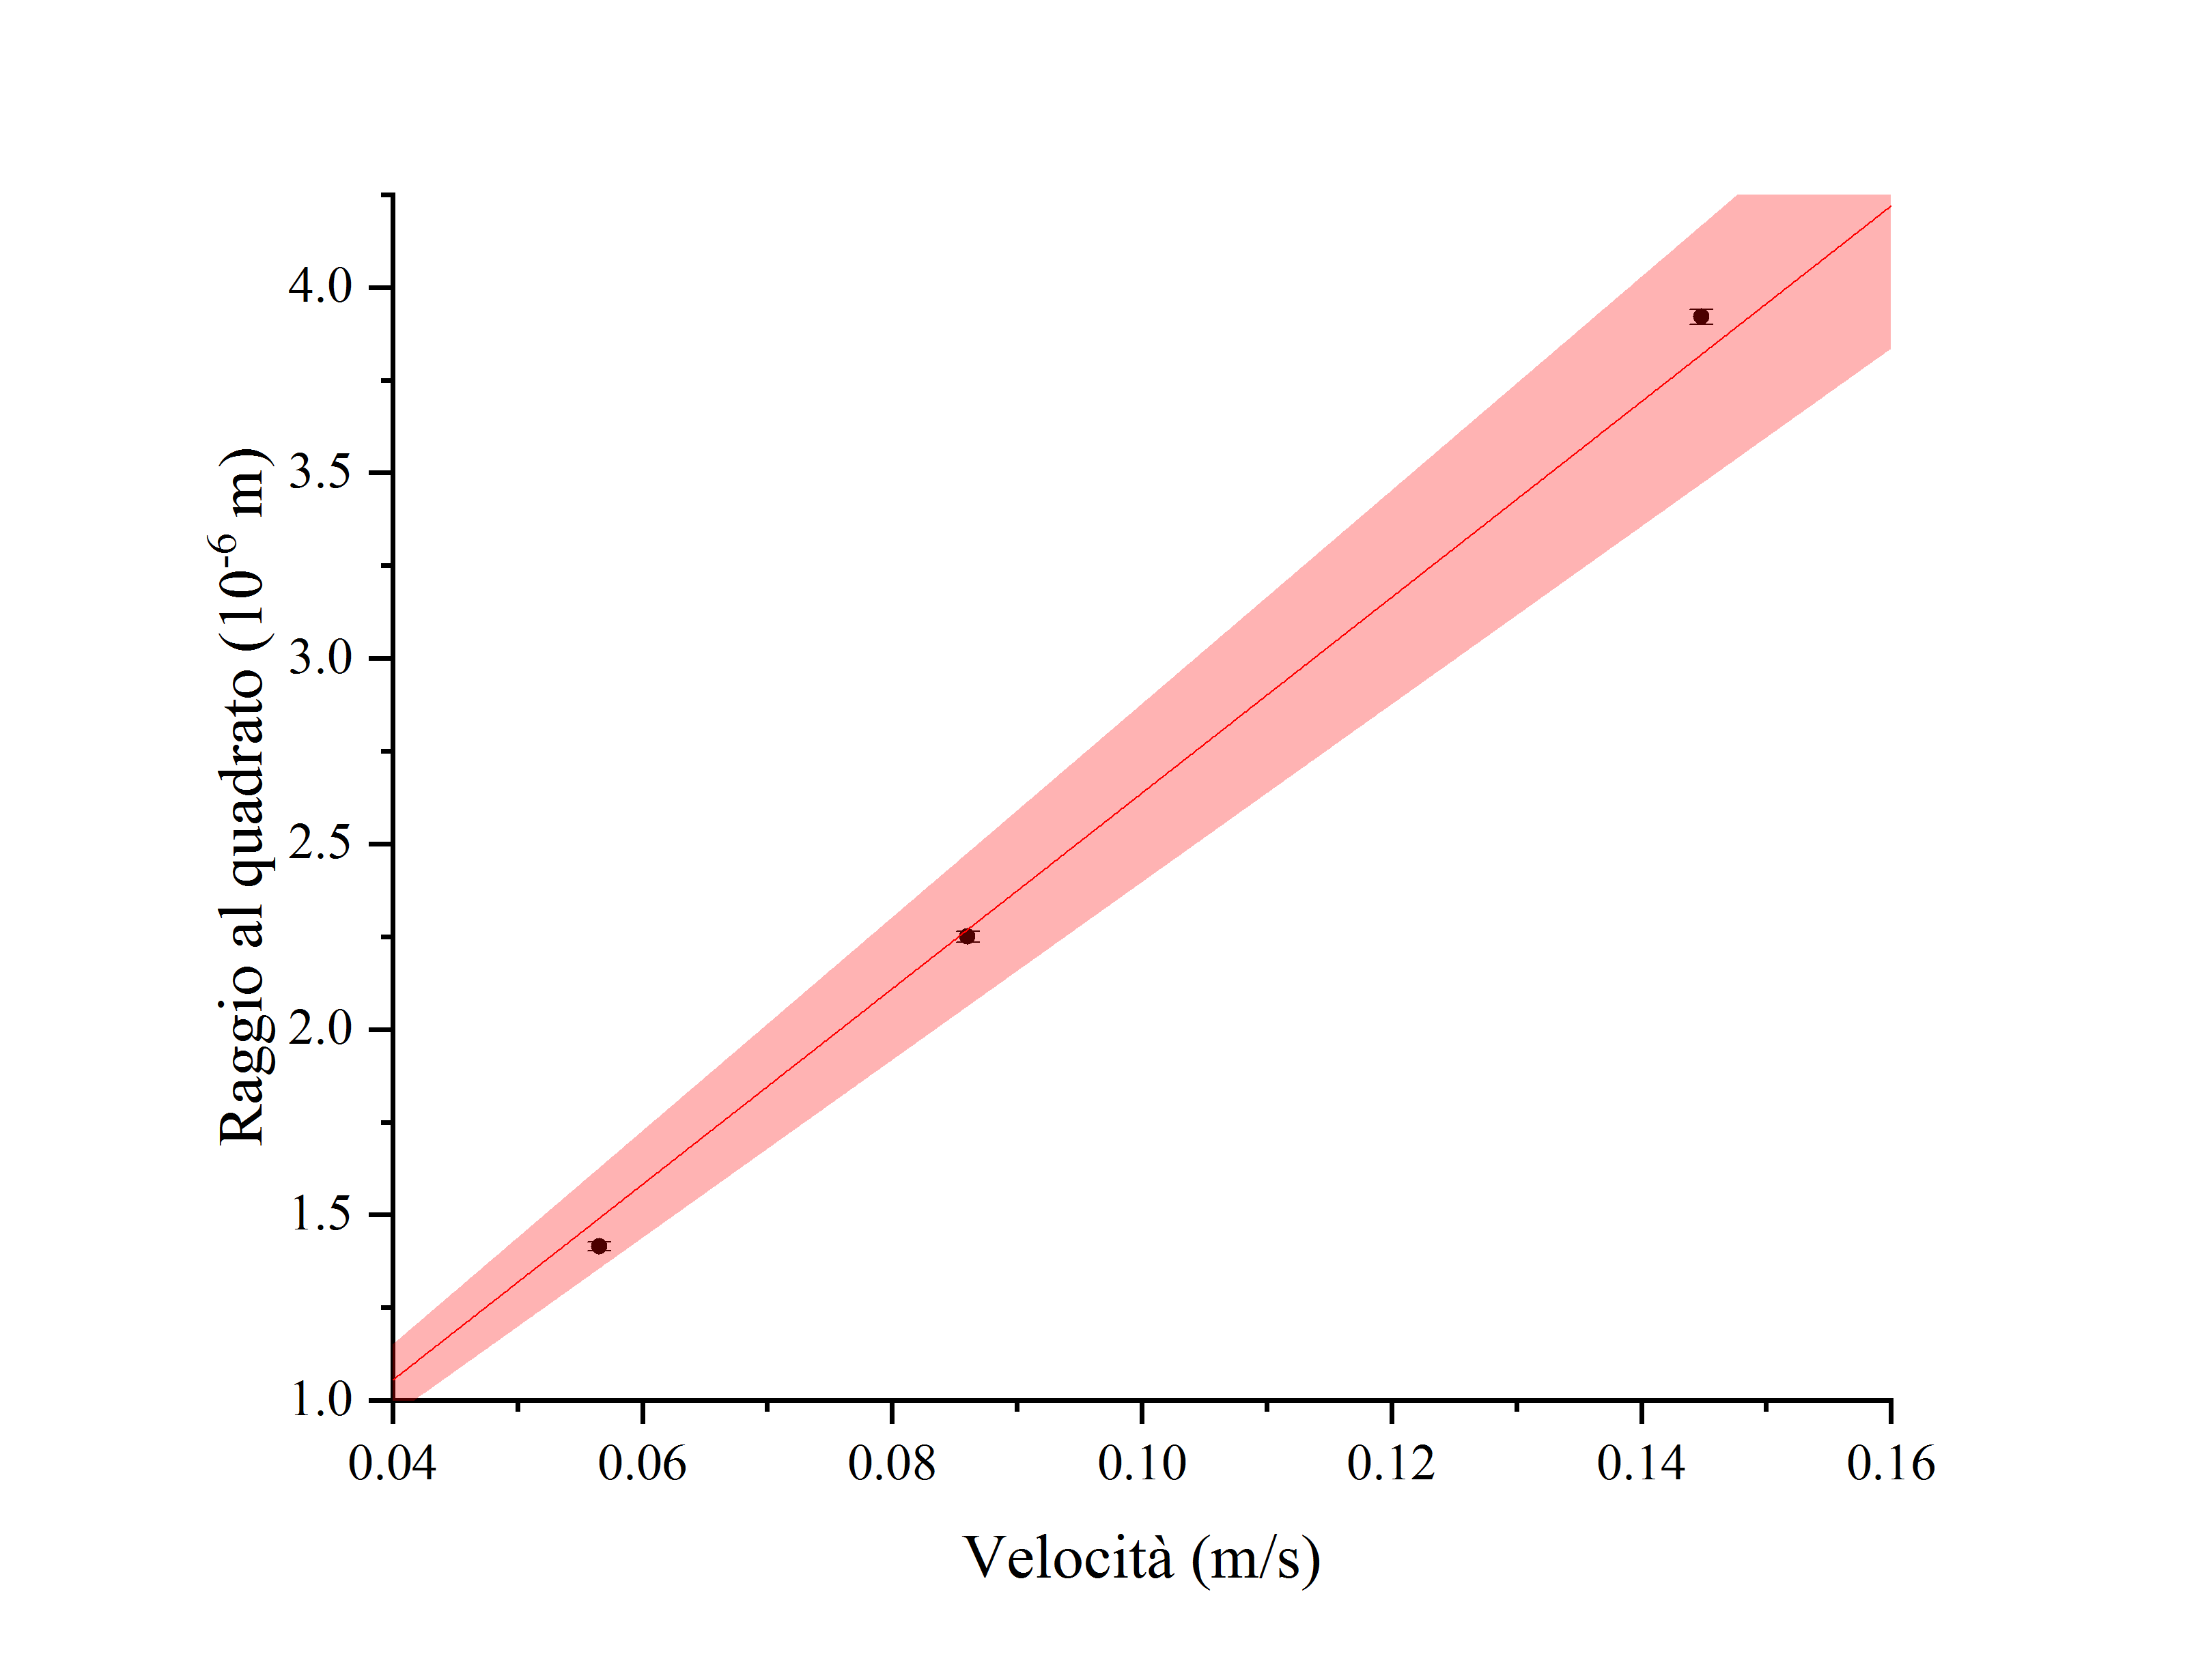
\includegraphics[trim={2.5cm 0.6cm 3cm 2.5cm},clip,width=.49\textwidth]{img/reg2.png}}
  \caption*{\emph{
    In rosso le rette di regressione, in rosa le rispettive
    regioni di incertezza.
    Le barre di errore in entrambe le direzioni sono riportate,
    ma sono troppo ridotte per poter essere apprezzate
    immediatamente.
  }}
\end{figure}

Per calcolare una prima stima di $\eta_\text{sol}$ è possibile approssimare
$\rho_\text{sol}\simeq\rho_\text{glicerina}$, calcolata in base
a $T_\text{amb}$ secondo il modello sopra citato:
\[
  \eta = \frac{2g(\rho_\text{sf} - \rho_\text{sol})}{9\xi}
  \simeq \frac{2g(\rho_\text{sf} -
    \rho_\text{glicerina}(T_\text{amb}))}{9\xi}
\]
I valori di $\eta_\text{sol}$ calcolati sulla base dei dati raccolti nelle
due giornate sono:
\[
  \eta_{\text{sol},1}=(256\pm3)\,\unit{mPa\,s}
  \qquad\qquad
  \eta_{\text{sol},2}=(371\pm4)\,\unit{mPa\,s}\]

\subsection{Concentrazione della glicerina}

Il modello empirico della viscosità di una soluzione acquosa di
glicerina\cite{Cheng2008} è descritto dalla seguente equazione:
\[
  \eta_\text{sol} =
    \eta_\text{acqua}^\alpha \eta_\text{glicerina}^{1-\alpha}
\]
al variare di un parametro $\alpha\in[0,1]$ legato alla
concentrazione dell'acqua. Risolvendo l'equazione in $\alpha$ si
ottiene:
\[
  \alpha = \frac{\ln{\eta_\text{sol}} - \ln{\eta_\text{glicerina}}}
    {\ln{\eta_\text{acqua}} - \ln{\eta_\text{glicerina}}}
\]
La relazione tra $\alpha$ e la concentrazione in massa $c_\text{m}$
della \emph{glicerina} in soluzione è invece la seguente:
\[
  \alpha = 1 - c_\text{m} + \frac{a b\,c_\text{m} (1 - c_\text{m})}
    {a\,c_\text{m} + b (1 - c_\text{m})}
  \qquad\text{con}\quad
  \begin{array}{l}
    a = 0.705 - 0.0017\,T_\text{amb} \\
    b = (4.9 + 0.036\,T_\text{amb})\,a^{2.5}
  \end{array}
\]
Risolvendo l'equazione in $c_\text{m}$ si ottiene:
\[
  c_\text{m} = \frac{
    -\alpha a + \alpha b + ab + a - 2b - \sqrt{\Delta}}{2(ab + a - b)}
\]
con $
\Delta = \alpha^2 a^2 - 2\alpha^2 ab + \alpha^2 b^2 - 2\alpha a^2 b -
2\alpha a^2 - 2\alpha a b^2 + 2\alpha ab + a^2 b^2 + 2a^2 b + a^2$.

\vspace{2mm}
I valori di $\alpha$ e $c_\text{m}$ calcolati a partire da $\eta_\text{sol}$ e
$T_\text{amb}$ per entrambi i giorni sono:
\[
\begin{aligned}
  \alpha_1 &= 0.174\pm0.006
  \qquad\qquad
  c_{\text{m},1} &= (93.6\pm0.3)\%\,\text{m}/\text{m}\\
  \alpha_2 &= 0.184\pm0.006
  \qquad\qquad
  c_{\text{m},2} &= (93.2\pm0.3)\%\,\text{m}/\text{m}\\
\end{aligned}
\]

\subsection{Ricalcolo della densità per una migliore stima}
Nota la concentrazione di glicerina, è ora possibile
calcolare una stima della densità della soluzione, facendo
ancora una volta affidamento al modello empirico\cite{Volk2018}:
\[
  \rho_\text{sol} = \kappa(T,c_\text{m}) \left(
  \rho_\text{acqua}(T) + \frac{
    \rho_\text{glicerina}(T) - \rho_\text{acqua}(T)
  }{1 + \frac{\rho_\text{glicerina}(T)}{\rho_\text{acqua}(T)}
    \!\left(\frac{1}{c_\text{m}} - 1\right)}
  \right)
\]
dove $
  \kappa(T,c_\text{m}) = 1 + \left(
    1.78\cdot10^{-6}\,T^2 - 1.82\cdot10^{-4}\,T + 1.41\cdot10^{-2}
  \right)\sin{\!\left(c_\text{m}^{1.31} \pi\right)}^{0.81}
$ è un coefficiente legato alla contrazione volumica, un fenomeno
osservabile sperimentalmente nella maggior parte delle miscele
liquide.

Applicando questa formula ai valori di $T$ e $c_\text{m}$ di cui
sopra, otteniamo:
\[
  \rho_{\text{sol},1} = (1241.5\pm1.2)\,\unit{kg \per m^2}
  \qquad\qquad
  \rho_{\text{sol},2} = (1243.7\pm1.2)\,\unit{kg \per m^2}
\]

Possiamo osservare facilmente che queste misure non sono compatibili
con i rispettivi valori di $\rho_\text{glicerina}$: l'approssimazione
$\rho_\text{sol} \simeq \rho_\text{glicerina}$ non è quindi
giustificata.

Tuttavia, è evidente che:
\[(\rho_\text{sol})_\text{best} < (\rho_\text{glicerina})_\text{best}\]

Si può allora immaginare che il $\rho_\text{sol}$ così determinato
approssimi il valore vero \emph{meglio} di $\rho_\text{glicerina}$:
il gruppo di lavoro ha quindi deciso di ricalcolare la densità della
soluzione come appena mostrato, utilizzando stavolta la nuova stima
di $\rho_\text{sol}$.

\vspace{2mm}

Reiterando questo processo più volte, le stime di
$\rho_\text{sol}$, $c_\text{m}$ ed $\eta_\text{sol}$ si sono
velocemente stabilizzate attorno a valori ben definiti:
di seguito riportiamo i risultati delle prime iterazioni.\footnote{
  Il gruppo di lavoro ha in realtà effettuato sei iterazioni:
  sono riportate soltanto le prime quattro, in quanto le
  differenze tra le successive si sono rivelate inapprezzabili.
}

\begin{center}\begin{tblr}{
  colspec={ |c|c|c|c|c| }
}
  \hline
  \textbf{Giorno 1}
    & $\rho_\text{sol}\;(\unit{kg\per m^3})$
    & $\eta_\text{sol}\;(\unit{mPa\,s})$ & $c_\text{m}\;(\%\,\text{m}/\text{m})$
    & $\rho_\text{sol}\;(\unit{kg\per m^3})$
    \\ Iterazione & (assunto) &&& (ottenuto) \\
  \hline
  1 & $1257.94\pm0.12$ & $256.42\pm2.99$ & $93.56\pm0.26$ & $1241.53\pm1.21$ \\
  \hline[dashed]
  2 & $1241.53\pm1.21$ & $257.08\pm3.03$ & $93.58\pm0.26$ & $1241.57\pm1.21$ \\
  \hline[dashed]
  3 & $1241.57\pm1.21$ & $257.07\pm3.03$ & $93.58\pm0.26$ & $1241.57\pm1.21$ \\
  \hline[dashed]
  4 & $1241.57\pm1.21$ & $257.07\pm3.03$ & $93.58\pm0.26$ & $1241.57\pm1.21$ \\
  \hline[dashed]
  $\vdots$ & $\vdots$ & $\vdots$ & $\vdots$ & $\vdots$ \\
\end{tblr}\end{center}
\begin{center}\begin{tblr}{
  colspec={ |c|c|c|c|c| }
}
  \hline
  \textbf{Giorno 2}
    & $\rho_\text{sol}\;(\unit{kg\per m^3})$
    & $\eta_\text{sol}\;(\unit{mPa\,s})$ & $c_\text{m}\;(\%\,\text{m}/\text{m})$
    & $\rho_\text{sol}\;(\unit{kg\per m^3})$
    \\ Iterazione & (assunto) &&& (ottenuto) \\
  \hline
  1 & $1261.13\pm0.12$ & $370.80\pm4.32$ & $93.17\pm0.25$ & $1243.73\pm1.17$ \\
  \hline[dashed]
  2 & $1243.73\pm1.17$ & $371.80\pm4.38$ & $93.18\pm0.25$ & $1243.77\pm1.17$ \\
  \hline[dashed]
  3 & $1243.77\pm1.17$ & $371.80\pm4.38$ & $93.19\pm0.25$ & $1243.77\pm1.17$ \\
  \hline[dashed]
  4 & $1243.77\pm1.17$ & $371.80\pm4.38$ & $93.19\pm0.25$ & $1243.77\pm1.17$ \\
  \hline[dashed]
  $\vdots$ & $\vdots$ & $\vdots$ & $\vdots$ & $\vdots$ \\
\end{tblr}\end{center}
\begin{center}
  \emph{
    \textbf{Nota.}
    Abbiamo riportato più cifre decimali del necessario,
    semplicemente per mostrare le piccole differenze tra
    le prime iterazioni.
  }
\end{center}

\textbf{Osservazione}. Possiamo ora calcolare il numero di Reynolds
(adimensionale) per ogni classe di sferette, alle due diverse temperature:

\begin{center}\begin{tblr}{ |c|c|c| }
  \hline
  Classe $k$ & $\text{Re}_k$, giorno 1 & $\text{Re}_k$, giorno 2 \\
  \hline
  Piccole & $33.8\pm0.9$ & $15.1\pm0.4$ \\
  \hline[dashed]
  Medie & $50.1\pm1.4$ & $23.0\pm0.7$ \\
  \hline[dashed]
  Grandi & $75.7\pm2.1$ & $38.8\pm1.1$ \\
  \hline
\end{tblr}\end{center}

È immediato osservare che tutti i valori di $\text{Re}_k$
calcolati soddisfano abbondantemente la condizione (2.1.2.):
l'applicazione di quel modello a questa esperienza è ora
pienamente giustificata.

\section{Conclusioni}

Sulla base dei dati acquisiti durante l'esperienza,
il gruppo di lavoro è riuscito a determinare la viscosità
e la concentrazione di una soluzione di acqua e glicerina.

Per valutare numericamente la compatibilità tra
$\eta_{\text{sol},1}$ ed $\eta_{\text{sol},2}$ (e tra
$c_{\text{m},1}$ e $c_{\text{m},2}$),
abbiamo calcolato i seguenti valori (numeri puri):
\[
  \varepsilon_\eta = \frac{
    \left|\left(\eta_{\text{sol},1}\right)_\text{best} -
    \left(\eta_{\text{sol},2}\right)_\text{best}\right|
  }{\delta\eta_{\text{sol},1} + \delta\eta_{\text{sol},2}}
\]\[
  \varepsilon_c = \frac{
    \left|\left(c_{\text{m},1}\right)_\text{best} -
    \left(c_{\text{m},2}\right)_\text{best}\right|
  }{\delta c_{\text{m},1} + \delta c_{\text{m},2}}
\]
Allora le due misure di $\eta_\text{sol}$ da noi ottenute
sono compatibili fra loro se e solo se $\varepsilon_\eta\le1$;
similmente, le due misure di $c_\text{m}$ sono compatibili
fra loro se e solo se $\varepsilon_c\le1$.

Nel nostro caso, $\varepsilon_\eta \simeq 0.923$
e $\varepsilon_c \simeq 0.758$: le due misure sono
dunque compatibili.

Possiamo pertanto affermare che l'esperienza si è
conclusa con successo.

\printbibliography

\end{document}
